% Compile from docs/latex with XeLaTeX. Shared formatting: common.tex.
% Options for packages loaded elsewhere
\PassOptionsToPackage{unicode}{hyperref}
\PassOptionsToPackage{hyphens}{url}
\documentclass[
  11pt,
]{article}
\usepackage{xcolor}
\usepackage[margin=1in]{geometry}
\usepackage{amsmath,amssymb}
\setcounter{secnumdepth}{-\maxdimen} % remove section numbering
\usepackage{iftex}
\ifPDFTeX
  \usepackage[T1]{fontenc}
  \usepackage[utf8]{inputenc}
  \usepackage{textcomp} % provide euro and other symbols
\else % if luatex or xetex
  \usepackage{unicode-math} % this also loads fontspec
  \defaultfontfeatures{Scale=MatchLowercase}
  \defaultfontfeatures[\rmfamily]{Ligatures=TeX,Scale=1}
\fi
\usepackage{lmodern}
\ifPDFTeX\else
  % xetex/luatex font selection
  \IfFontExistsTF{Times New Roman}{\setmainfont{Times New Roman}}{\setmainfont{TeX Gyre Termes}}
\fi
% Use upquote if available, for straight quotes in verbatim environments
\IfFileExists{upquote.sty}{\usepackage{upquote}}{}
\IfFileExists{microtype.sty}{% use microtype if available
  \usepackage[]{microtype}
  \UseMicrotypeSet[protrusion]{basicmath} % disable protrusion for tt fonts
}{}
\makeatletter
\@ifundefined{KOMAClassName}{% if non-KOMA class
  \IfFileExists{parskip.sty}{%
    \usepackage{parskip}
  }{% else
    \setlength{\parindent}{0pt}
    \setlength{\parskip}{6pt plus 2pt minus 1pt}}
}{% if KOMA class
  \KOMAoptions{parskip=half}}
\makeatother
\usepackage{longtable,booktabs,array}
\usepackage{caption}
\captionsetup[longtable]{position=bottom,skip=5pt,font={scriptsize,it},width=\linewidth,justification=centering}
\newcounter{none} % for unnumbered tables
\usepackage{calc} % for calculating minipage widths
% Correct order of tables after \paragraph or \subparagraph
\usepackage{etoolbox}
\makeatletter
\patchcmd\longtable{\par}{\if@noskipsec\mbox{}\fi\par}{}{}
\makeatother
\usepackage{graphicx}
\makeatletter
\newsavebox\pandoc@box
\newcommand*\pandocbounded[1]{% scales image to fit in text height/width
  \sbox\pandoc@box{#1}%
  \Gscale@div\@tempa{\textheight}{\dimexpr\ht\pandoc@box+\dp\pandoc@box\relax}%
  \Gscale@div\@tempb{\linewidth}{\wd\pandoc@box}%
  \ifdim\@tempb\p@<\@tempa\p@\let\@tempa\@tempb\fi% select the smaller of both
  \ifdim\@tempa\p@<\p@\scalebox{\@tempa}{\usebox\pandoc@box}%
  \else\usebox{\pandoc@box}%
  \fi%
}
% Set default figure placement to htbp
\def\fps@figure{htbp}
\makeatother
\setlength{\emergencystretch}{3em} % prevent overfull lines
\providecommand{\tightlist}{%
  \setlength{\itemsep}{0pt}\setlength{\parskip}{0pt}}
\usepackage{bookmark}
\IfFileExists{xurl.sty}{\usepackage{xurl}}{} % add URL line breaks if available
\urlstyle{same}
% fallback for those not using the hyperref driver hyperxmp:
\makeatletter
\@ifundefined{xmpquote}{\newcommand{\xmpquote}[1]{#1}}{}
\makeatother
\hypersetup{
  hidelinks,
  pdfcreator={LaTeX via pandoc}}



% Shared layout based on the Word test plan.
\usepackage{sectsty}
\sectionfont{\fontsize{14}{17}\selectfont}
\subsectionfont{\fontsize{12}{15}\selectfont}
\subsubsectionfont{\fontsize{11}{14}\selectfont}
\AtBeginEnvironment{longtable}{\fontsize{8.5}{10.5}\selectfont}
\newcommand{\projecttitle}[1]{\begin{center}{\fontsize{22}{26}\selectfont #1\par}\end{center}}
\newcommand{\documentsubtitle}[1]{\begin{center}{\fontsize{15}{18}\selectfont #1\par}\end{center}}

\renewcommand{\contentsname}{Table of Contents}
\makeatletter
\renewcommand*\l@section[2]{\@dottedtocline{1}{0em}{0em}{\textbf{#1}}{#2}}
\renewcommand*\l@subsection[2]{\@dottedtocline{2}{1.5em}{0em}{\normalfont #1}{#2}}
\makeatother

\usepackage{tikz}

\begin{document}

\projecttitle{AI-Driven Pharmaceutical Real-Time Inventory and Customer Information System}

\documentsubtitle{Software Design Specification Document}

\begin{center}{\fontsize{12}{14}\selectfont\itshape Draft: Version 0.2\par}\end{center}

Course: Software Engineering

Team: Seal-SIMD

Team Members: Maria Molano Escobar, Marko Maksuti, Ryan Petillo, Samuel Cordova

Instructor: Hubert Johnson

Date: November 28, 2026

\clearpage
{\def\LTcaptype{none} % do not increment counter
\begin{longtable}[]{|
  >{\raggedright\arraybackslash}m{(\linewidth - 4\tabcolsep - 3\arrayrulewidth) * \real{0.4749}}|
  >{\raggedright\arraybackslash}m{(\linewidth - 4\tabcolsep - 3\arrayrulewidth) * \real{0.4765}}|}
\hline
\begin{minipage}[c]{\linewidth}\raggedright
\textbf{Document control}
\end{minipage} & \begin{minipage}[c]{\linewidth}\raggedright
\textbf{Value}
\end{minipage} \\
\hline
\endhead

\endlastfoot
Team & Seal-SIMD \\ \hline
Contributors (SRS team) & Maria Molano Escobar; Marko Maksuti; Ryan Petillo; Samuel Cordova \\ \hline
Course/instructor & CSIT 515 Software Engineering \& Reliability / Dr. Hubert Johnson \\ \hline
Due date & October 29, 2026 (Week 8) \\ \hline
Version & 0.2 --- revised detailed design draft \\ \hline
Baseline & Software Requirements Specification v0.3, November 10, 2026 \\ \hline
Section authors/module owners & To be assigned and confirmed by team; do not infer individual contributions \\ \hline
\end{longtable}
}

\clearpage
\tableofcontents

\clearpage
\section{1. Introduction}\label{introduction}

\subsection{1.1 Purpose of this document}\label{purpose-of-this-document}

This document will define the detailed software design for the AI-Driven Pharmaceutical Real-Time Inventory and Customer Information System. It will translate the approved requirements into architecture, domain classes, persistent entities, module responsibilities, interfaces, algorithms, error handling, security controls and use-case realizations. A developer will be able to use these contracts together with the requirements specification to implement the system without inventing additional business rules.

\subsection{1.2 Purpose of the system}\label{purpose-of-the-system}

The system will provide a Pharmacy Operations application for authenticated staff and a Customer Information Portal for customers. Pharmacy staff will receive and issue stock by documented product lots, calculate stock from immutable GRN and GIN lines, perform approved corrections, manage expiration and purchase orders, and review forecasts and recommendations. Customers will search medications, view safe availability and cash prices, locate participating pharmacies and optionally request back-in-stock notices.

\subsection{1.3 Scope and design basis}\label{scope-and-design-basis}

The first implementation will prioritize the working, auditable inventory kernel and the required demonstration paths. This design will use the Software Requirements Specification v0.3 as its behavioral baseline. Design decisions will not weaken or silently replace a requirement; any later scope or behavior change will require corresponding updates to both documents.

\clearpage
\section{2. Detailed Design Scope, Assumptions and Decisions}\label{system-scope-assumptions-and-decisions}

\subsection{2.1 Core deliverable and extensions}\label{core-deliverable-and-extensions}

{\def\LTcaptype{none} % do not increment counter
\begin{longtable}[]{|
  >{\raggedright\arraybackslash}m{(\linewidth - 6\tabcolsep - 4\arrayrulewidth) * \real{0.3116}}|
  >{\raggedright\arraybackslash}m{(\linewidth - 6\tabcolsep - 4\arrayrulewidth) * \real{0.3292}}|
  >{\raggedright\arraybackslash}m{(\linewidth - 6\tabcolsep - 4\arrayrulewidth) * \real{0.3116}}|}
\hline
\begin{minipage}[c]{\linewidth}\raggedright
\textbf{Package}
\end{minipage} & \begin{minipage}[c]{\linewidth}\raggedright
\textbf{Included behavior}
\end{minipage} & \begin{minipage}[c]{\linewidth}\raggedright
\textbf{Priority/strategy}
\end{minipage} \\
\hline
\endhead

\endlastfoot
Kernel K0 & Products, stores, lots, atomic stock movements, authentication/roles, audit, expiration and sale blocking, staff read screens, customer safe search, durable offline transaction queue and reconnection synchronization & First: integrated skeleton \\ \hline
Operational K1 & Supplier and reorder thresholds, draft orders and manager approval, dashboard, POS adapter & Next \\ \hline
Analytics K2 & Sales history, forecast interface, 7/30/90 day baseline model, suggestions requiring approval & Next; degrade to rules when model unavailable \\ \hline
Extensions E1 & Cycle counts, supplier transmission, disposal/FEFO, export reports, back-in-stock and generic alternatives & Only after kernel works \\ \hline
Extensions E2 & Advanced chatbot and embedded map integration; the nearby-pharmacy list and offline transaction synchronization remain required & Scoped prototype or deferred \\ \hline
\end{longtable}
}

\subsection{2.2 Exclusions inherited from SRS}\label{exclusions-inherited-from-srs}

The prototype will use manual receiving and one inventory per pharmacy, broken down by product and lot. Barcode scanning, warehouse or room balances, location transfers, dispensing, e-prescribing, insurance claims, payments, home delivery and medical or dosing advice will remain outside scope. Customer search will never expose exact inventory counts. Schedule II availability will be replaced by a contact-pharmacy message.

\subsection{2.3 Cross-cutting design decisions}\label{cross-cutting-decisions-requiring-team-approval}

\begin{quote}
· The implementation will use a TypeScript npm workspace: React and Vite for the client, Express for the server, shared TypeScript contracts, SQLite through better-sqlite3 for the prototype database, Zod for request validation and Vitest for automated tests.

· The database will be the source of truth for inventory; the ML/chat layer will not write inventory or authorize purchase orders.

· Every stock-changing command will use a server-side database transaction, and every external event will carry a stable idempotency key.

· The classroom prototype will not claim HIPAA or DSCSA certification; it will implement the specified safeguards and will identify production compliance work as outside scope.

· Demonstrations will use synthetic medication, inventory, user and sales data and will contain no real customer medical information.
\end{quote}





\clearpage
\section{3. Overall Architecture and Deployment}\label{overall-architecture-and-deployment}

\begin{center}
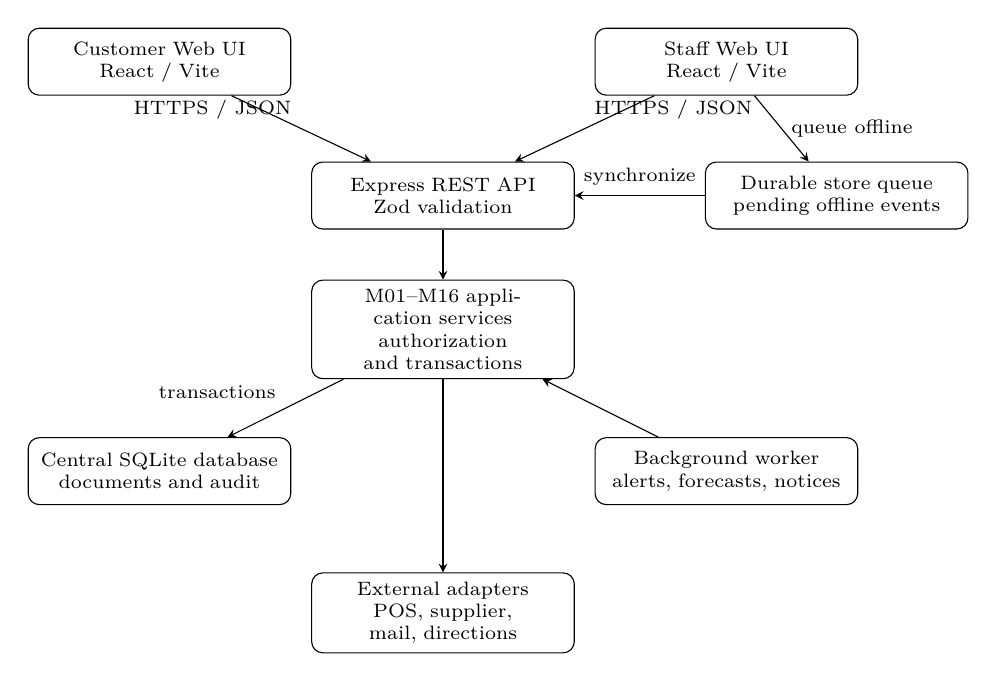
\begin{tikzpicture}[font=\scriptsize,component/.style={draw,rounded corners,align=center,text width=3.1cm,minimum height=.85cm},link/.style={-stealth}]
\node[component] (customer) at (-3.6,4.4) {Customer Web UI\\React / Vite};
\node[component] (staff) at (3.6,4.4) {Staff Web UI\\React / Vite};
\node[component] (api) at (0,2.7) {Express REST API\\Zod validation};
\node[component] (queue) at (5.0,2.7) {Durable store queue\\pending offline events};
\node[component] (services) at (0,1.0) {M01--M16 application services\\authorization and transactions};
\node[component] (db) at (-3.6,-.8) {Central SQLite database\\documents and audit};
\node[component] (worker) at (3.6,-.8) {Background worker\\alerts, forecasts, notices};
\node[component] (external) at (0,-2.6) {External adapters\\POS, supplier, mail, directions};
\draw[link] (customer) -- node[above left]{HTTPS / JSON} (api);
\draw[link] (staff) -- node[above right]{HTTPS / JSON} (api);
\draw[link] (staff) -- node[right]{queue offline} (queue);
\draw[link] (queue) -- node[above]{synchronize} (api);
\draw[link] (api) -- (services);
\draw[link] (services) -- node[above left]{transactions} (db);
\draw[link] (worker) -- (services);
\draw[link] (services) -- (external);
\end{tikzpicture}
\end{center}

\subsection{3.1 Implementation technology}\label{implementation-technology}

The repository will use Node.js 20 or later and npm workspaces. The client will use React, React Router and Vite. The staff client will persist offline transactions in IndexedDB before displaying them as pending synchronization. The server will use Express and Zod. Shared request, response and domain types will be published by the shared workspace. The demonstration database will use SQLite through better-sqlite3; repository interfaces will isolate SQL from application services. Vitest and Testing Library will provide automated tests.

\subsection{3.2 Separation and dependencies}\label{separation-and-dependencies}

User interfaces will call API application services rather than the database. Application services will invoke repository abstractions and authorization checks; every inventory change will use M03, M04, M05 or M06 to create an immutable GRN or GIN. External systems will connect through adapters. Search will derive a safe public projection rather than query raw lots. The forecasting service will consume historical aggregates and return advisory objects only.

\subsection{3.3 Component dependency rules}\label{component-dependency-rules}

{\def\LTcaptype{none} % do not increment counter
\begin{longtable}[]{|
  >{\raggedright\arraybackslash}m{(\linewidth - 4\tabcolsep - 3\arrayrulewidth) * \real{0.4733}}|
  >{\raggedright\arraybackslash}m{(\linewidth - 4\tabcolsep - 3\arrayrulewidth) * \real{0.4781}}|}
\hline
\begin{minipage}[c]{\linewidth}\raggedright
\textbf{Caller}
\end{minipage} & \begin{minipage}[c]{\linewidth}\raggedright
\textbf{Allowed dependencies}
\end{minipage} \\
\hline
\endhead

\endlastfoot
Staff UI / customer UI & HTTP API contracts only \\ \hline
Inventory, Ordering, Expiration & Product, Store, Repository, Auth context, Audit \\ \hline
Public Search & Product public projection, Availability classifier, Store lookup \\ \hline
Forecast service & Read-only Sales History and Inventory snapshots \\ \hline
Adapters & Will use only published integration ports and will not write stock directly \\ \hline
Jobs & Application-service commands with service identity and audited outcomes \\ \hline
\end{longtable}
}

\subsection{3.4 Deployment and failure boundaries}\label{deployment-and-failure-boundaries}

For a semester prototype, one backend instance, one relational database, and a worker process will be sufficient. The UI will show an explicit last-updated timestamp. A temporary failed POS connection will be queued and retried with the same event ID and will not be counted twice. When the ML service is unavailable, manual reorder thresholds and the inventory kernel will remain usable. A future deployment may separate workers and add redundancy without changing public contracts.









\clearpage
\section{4. Design Conventions and Global Contracts}\label{design-conventions-and-global-contracts}

{\def\LTcaptype{none} % do not increment counter
\begin{longtable}[]{|
  >{\raggedright\arraybackslash}m{(\linewidth - 4\tabcolsep - 3\arrayrulewidth) * \real{0.4765}}|
  >{\raggedright\arraybackslash}m{(\linewidth - 4\tabcolsep - 3\arrayrulewidth) * \real{0.4749}}|}
\hline
\begin{minipage}[c]{\linewidth}\raggedright
\textbf{Convention}
\end{minipage} & \begin{minipage}[c]{\linewidth}\raggedright
\textbf{Rule}
\end{minipage} \\
\hline
\endhead

\endlastfoot
Identifiers & UUID-like opaque IDs; NDC remains a string (preserve leading zeros) \\ \hline
Pharmacy scope & Store will represent one participating pharmacy and its single inventory; it will not represent a warehouse or room within that pharmacy \\ \hline
Time & Store timestamps in UTC; display local pharmacy time; a lot will become unsellable at 00:00 on its expiration date in the pharmacy's local timezone \\ \hline
Money & Decimal cents or fixed decimal; never binary floating-point for money \\ \hline
Quantities & Nonnegative integer on-hand; net receipt and issue quantities with atomic checks \\ \hline
Public availability & Will be Out of Stock when calculated sellable stock is 0, Low Stock when it is positive and at or below the pharmacy's low-stock threshold, and In Stock when it is above that threshold \\ \hline
API responses & JSON result \{data, requestId\} or \{error: \{code, message, details\}, requestId\} \\ \hline
Authorization & Server enforces role and store scope on every operation \\ \hline
Versioning & Proposed /api/v1/*; breaking changes require a new version \\ \hline
Mutation retries & Idempotency key for POS, stock receipt, and approved external transmissions \\ \hline
Concurrency & Atomic compare-and-update or row lock for lot decrement \\ \hline
Pagination & Cursor or bounded page limit; default 25, max 100 \\ \hline
\end{longtable}
}

\subsection{4.1 Common state and invariant definitions}\label{common-state-and-invariant-definitions}

\begin{quote}
· Available-to-sell = sum of active, unexpired, non-quarantined lot quantities in a store; do not promise availability from stale inventory.

· A GRN is generated after delivery inspection and is immutable. A later delivery generates another GRN linked to the same purchase order and purchase invoice.

· Only authorized pharmacist/manager approval transitions a pending adjustment or purchase order to approved.

· Every GRN or GIN and its corresponding audit event will be committed in one transaction.

· M08 will flag unusual inventory activity when one pharmacy-product's total GRN plus GIN quantity for a local calendar day exceeds both five units and three times its mean daily movement during the preceding 30 complete days. Replayed event identifiers will contribute no additional quantity.

· M08 will flag an expiration risk when forecast demand through a lot's expiration date, after allocation to earlier-expiring lots, is lower than that lot's calculated on-hand quantity. The warning will show the lot quantity, expiration date, forecast horizon and forecast units used.

· An expired lot cannot be selected for sale, even if an earlier search result showed stock.
\end{quote}

\subsection{4.2 Shared error catalog}\label{shared-error-catalog}

{\def\LTcaptype{none} % do not increment counter
\begin{longtable}[]{|
  >{\raggedright\arraybackslash}m{(\linewidth - 4\tabcolsep - 3\arrayrulewidth) * \real{0.4957}}|
  >{\raggedright\arraybackslash}m{(\linewidth - 4\tabcolsep - 3\arrayrulewidth) * \real{0.4556}}|}
\hline
\begin{minipage}[c]{\linewidth}\raggedright
\textbf{Error}
\end{minipage} & \begin{minipage}[c]{\linewidth}\raggedright
\textbf{Cause/responsee}
\end{minipage} \\
\hline
\endhead

\endlastfoot
VALIDATION\_ERROR & Field missing, malformed, or out of range; 400 \\ \hline
UNAUTHENTICATED & No valid staff session; 401 \\ \hline
FORBIDDEN & Role or store access denied; 403 \\ \hline
NOT\_FOUND & Resource absent or hidden; 404 \\ \hline
CONFLICT & Concurrent modification, duplicate or invalid state; 409 \\ \hline
INSUFFICIENT\_STOCK & Sale exceeds sellable quantity; 409 \\ \hline
EXPIRED\_LOT & Attempted sale of expired lot; 409 \\ \hline
DEPENDENCY\_UNAVAILABLE & POS, supplier, forecast, or map service unavailable; 503 \\ \hline
INTERNAL\_ERROR & Unexpected failure; generic public response and internal correlation ID; 500 \\ \hline
\end{longtable}
}








\clearpage
\section{5. Data Model and Invariants}\label{data-model-and-invariants}

Proposed normalized relational entities. Unique keys and constraints are design requirements; exact DDL depends on the team's database selection.

{\def\LTcaptype{none} % do not increment counter
\begin{longtable}[]{|
  >{\raggedright\arraybackslash}m{(\linewidth - 6\tabcolsep - 4\arrayrulewidth) * \real{0.3196}}|
  >{\raggedright\arraybackslash}m{(\linewidth - 6\tabcolsep - 4\arrayrulewidth) * \real{0.3244}}|
  >{\raggedright\arraybackslash}m{(\linewidth - 6\tabcolsep - 4\arrayrulewidth) * \real{0.3084}}|}
\hline
\begin{minipage}[c]{\linewidth}\raggedright
\textbf{Entity}
\end{minipage} & \begin{minipage}[c]{\linewidth}\raggedright
\textbf{Key fields}
\end{minipage} & \begin{minipage}[c]{\linewidth}\raggedright
\textbf{Responsibility}
\end{minipage} \\
\hline
\endhead

\endlastfoot
Store & id PK, name, address, postal\_code, latitude?, longitude?, timezone, active & Owns inventory and public search location \\ \hline
User & id PK, username unique, email, password\_hash, mfa\_enabled, status & Staff login principal \\ \hline
RoleAssignment & id PK, user\_id FK, store\_id FK, role & Scopes privilege to store \\ \hline
Customer & id PK, email unique, password\_hash, verified\_at, status & Optional registered-customer account \\ \hline
Product & id PK, ndc unique, brand\_name, generic\_name, strength, form, category, schedule\_class, active & Canonical catalog \\ \hline
StoreProduct & id PK, store\_id FK, product\_id FK, cash\_price, reorder\_point, low\_stock\_threshold, active & Per-store listing and settings \\ \hline
Supplier & id PK, name, contact, lead\_days, minimum\_order & Procurement master \\ \hline
Lot & id PK, store\_product\_id FK, supplier\_id FK, lot\_number, expires\_on, status, version & Lots and safety/expiry \\ \hline
LotStock (SQL view) & store\_id, product\_id, lot\_id, on\_hand & Sum GRNLine quantities minus sum GINLine quantities; invoices and audit records will not affect stock \\ \hline
PurchaseInvoice & id PK, number, supplier\_id FK, purchase\_order\_id FK, invoice\_date, currency, subtotal, tax, total & Supplier charge document; will not affect stock \\ \hline
PurchaseInvoiceLine & id PK, purchase\_invoice\_id FK, product\_id FK, quantity, unit\_price, tax, line\_total & Purchase-invoice line values \\ \hline
SalesInvoice & id PK, number, customer\_id FK?, store\_id FK, sales\_event\_id FK unique, invoice\_date, currency, subtotal, tax, total & Customer charge document; will not affect stock \\ \hline
SalesInvoiceLine & id PK, sales\_invoice\_id FK, product\_id FK, quantity, unit\_price, tax, line\_total & Sales-invoice line values \\ \hline
GRN & id PK, number, store\_id FK, purchase\_order\_id FK?, purchase\_invoice\_id FK?, adjustment\_request\_id FK?, source, created\_by, created\_at & Immutable receipt header; source will be DELIVERY or CORRECTION \\ \hline
GRNLine & id PK, grn\_id FK, product\_id FK, lot\_id FK, expiration\_date, quantity & Immutable positive stock receipt quantity \\ \hline
GIN & id PK, number, store\_id FK, sales\_invoice\_id FK?, adjustment\_request\_id FK?, source, reason, created\_by, created\_at & Immutable issue header; source will be SALE, DISPOSAL, SUPPLIER\_RETURN or CORRECTION \\ \hline
GINLine & id PK, gin\_id FK, product\_id FK, lot\_id FK, quantity & Immutable positive stock issue quantity \\ \hline
DeliveryCheck & id PK, purchase order FK, purchase invoice FK, store FK, result, checked by, checked at, confirmed by, confirmed at, explanation & Will preserve the physical inspection and its correct or incorrect result before GRN generation. \\ \hline
DeliveryCheckLine & id PK, delivery check FK, product, lot, expiration date, physical quantity, discrepancy type, kept quantity & Discrepancy type will be extra product, missing product, expired product or quantity difference. \\ \hline
AdjustmentRequest & id PK, lot\_id FK, calculated\_quantity, counted\_quantity, reason\_code, explanation, status, requested\_by, reviewed\_by?, resulting\_grn\_id?, resulting\_gin\_id? & Approval workflow that will produce one correction GRN or GIN \\ \hline
PurchaseOrder & id PK, store\_id FK, supplier\_id FK, status, created\_by, approved\_by?, created\_at & Ordering \\ \hline
PurchaseOrderLine & id PK, order\_id FK, product\_id FK, qty, unit\_price & Order line items \\ \hline
SalesEvent & id PK, external\_event\_id unique, store\_id FK, sold\_at, status & Idempotent sale header \\ \hline
SalesEventLine & id PK, sales\_event\_id FK, product\_id FK, quantity, unit\_price, tax & One product line received from the POS system \\ \hline
Forecast & id PK, store\_product\_id FK, horizon\_days, predicted\_units, generated\_at, model\_version, quality? & Advisory output \\ \hline
Recommendation & id PK, store\_product\_id FK, suggested\_qty, reason, status, reviewer\_id? & Requires human decision \\ \hline
AuditEvent & id PK, actor\_id?, store\_id?, action, entity\_type, entity\_id, before\_json?, after\_json?, at & Audit trail \\ \hline
Alert & id PK, store\_id, alert\_type, resource\_id, severity, created\_at, viewed\_at? & Expiration / low-stock \\ \hline
Subscription & id PK, customer\_id, store\_product\_id, status & Optional customer notification \\ \hline
OfflineTransaction & id PK, store\_id FK, event\_id unique, event\_type, payload, expected\_version, created\_at, synchronization\_status & Durable local event awaiting central acknowledgement \\ \hline
SynchronizationConflict & id PK, offline\_transaction\_id FK, server\_version, conflict\_code, detected\_at, resolved\_at? & Explicit version conflict requiring staff action \\ \hline
\end{longtable}
}

\subsection{5.1 Primary relationships}\label{primary-relationships}

M04 will calculate stock through the LotStock SQL view. For each pharmacy, product and lot, the view will sum GRNLine quantities and subtract GINLine quantities. No service will store or directly update an on-hand balance. Lot will store identity and expiration metadata only. A stock-changing transaction will create the applicable immutable GRN or GIN, its lines and the audit event atomically.

M03 will compare the technician's physical delivery entries with the purchase order and linked purchase invoice. A correct delivery will immediately generate an immutable GRN. An extra product, missing product, expired product or confirmed quantity difference will record an incorrect delivery. The technician may edit and recount a different quantity repeatedly before confirming it. For an incorrect delivery, a Pharmacist / Manager will confirm the physical quantities of ordered, unexpired products that the pharmacy will keep and will enter an explanation; M03 will exclude returned extra and expired products and will generate one GRN containing the kept quantities. Stock will change only when that GRN is created. Received purchase-order quantity will equal the sum of its linked GRN quantities, so 8 units received today and 2 tomorrow will create separate GRNs for 8 and 2 without editing either document.

An approved physical-count correction will preserve the entered count, calculated quantity, reason and manager decision. If the counted quantity is greater, M05 will create one correction GRN for the difference. If it is lower, M05 will create one correction GIN for the difference. If it is equal, M05 will record the completed count without creating an inventory note. This rule will preserve the SRS stock formula for every correction.

Store 1:N StoreProduct; Product 1:N StoreProduct; StoreProduct 1:N Lot; Lot 1:N GRNLine and GINLine; Store 1:N PurchaseOrder; PurchaseOrder 1:N PurchaseOrderLine; PurchaseOrder 1:N PurchaseInvoice and GRN; PurchaseInvoice 1:N PurchaseInvoiceLine and 1:N GRN; GRN 1:N GRNLine; GIN 1:N GINLine; DeliveryCheck 1:N DeliveryCheckLine; SalesEvent 1:N SalesEventLine and 1:1 SalesInvoice; SalesInvoice 1:N SalesInvoiceLine and 1:1 GIN for an accepted sale; Customer 1:N Subscription; Store 1:N OfflineTransaction. User N:M Store through RoleAssignment. AuditEvent will refer to its target by type and ID.

\subsection{5.2 Domain class relationships}\label{domain-class-relationships}

\begin{center}
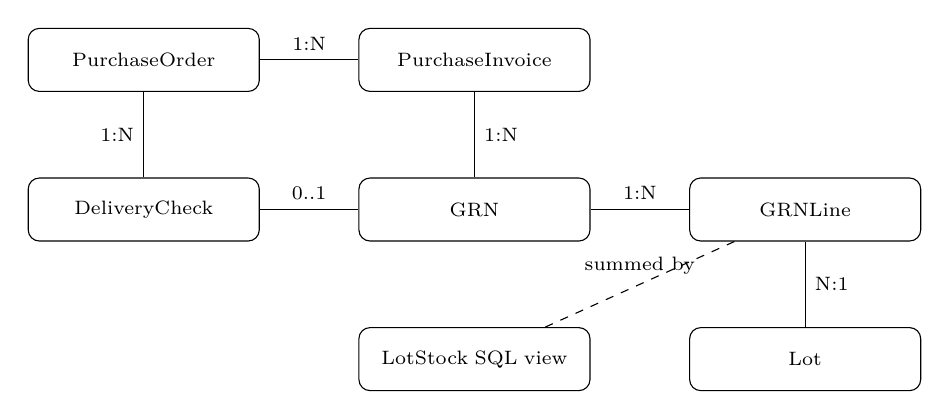
\begin{tikzpicture}[font=\scriptsize,entity/.style={draw,rounded corners,align=center,text width=2.7cm,minimum height=.8cm},rel/.style={}]
\node[entity] (po) at (0,3.6) {PurchaseOrder};
\node[entity] (pi) at (4.2,3.6) {PurchaseInvoice};
\node[entity] (check) at (0,1.7) {DeliveryCheck};
\node[entity] (grn) at (4.2,1.7) {GRN};
\node[entity] (grnl) at (8.4,1.7) {GRNLine};
\node[entity] (lot) at (8.4,-.2) {Lot};
\node[entity] (stock) at (4.2,-.2) {LotStock SQL view};
\draw[rel] (po) -- node[above]{1:N} (pi);
\draw[rel] (po) -- node[left]{1:N} (check);
\draw[rel] (pi) -- node[right]{1:N} (grn);
\draw[rel] (check) -- node[above]{0..1} (grn);
\draw[rel] (grn) -- node[above]{1:N} (grnl);
\draw[rel] (grnl) -- node[right]{N:1} (lot);
\draw[rel,dashed] (grnl) -- node[above]{summed by} (stock);
\end{tikzpicture}
\end{center}

\begin{center}
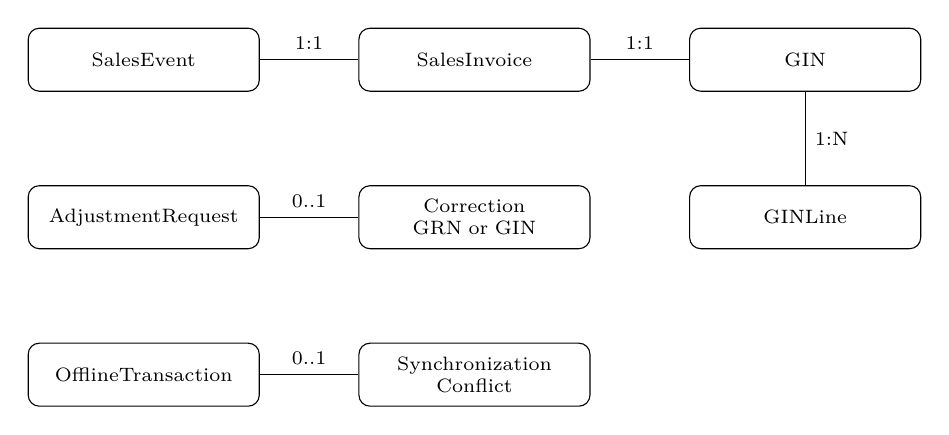
\begin{tikzpicture}[font=\scriptsize,entity/.style={draw,rounded corners,align=center,text width=2.7cm,minimum height=.8cm},rel/.style={}]
\node[entity] (sale) at (0,3.5) {SalesEvent};
\node[entity] (invoice) at (4.2,3.5) {SalesInvoice};
\node[entity] (gin) at (8.4,3.5) {GIN};
\node[entity] (ginl) at (8.4,1.5) {GINLine};
\node[entity] (adjust) at (0,1.5) {AdjustmentRequest};
\node[entity] (correction) at (4.2,1.5) {Correction GRN or GIN};
\node[entity] (offline) at (0,-.5) {OfflineTransaction};
\node[entity] (conflict) at (4.2,-.5) {Synchronization\\Conflict};
\draw[rel] (sale) -- node[above]{1:1} (invoice);
\draw[rel] (invoice) -- node[above]{1:1} (gin);
\draw[rel] (gin) -- node[right]{1:N} (ginl);
\draw[rel] (adjust) -- node[above]{0..1} (correction);
\draw[rel] (offline) -- node[above]{0..1} (conflict);
\end{tikzpicture}
\end{center}

\subsection{5.3 Constraints}\label{constraints}

\begin{quote}
· GRNLine and GINLine quantities will be positive whole numbers; calculated LotStock will never become negative; purchase-order quantities will be positive; cash price will be nonnegative; forecast horizon will be one of 7, 30 or 90 days.

· For each lot, (store\_product\_id, lot\_number, supplier\_id) is unique unless a merge policy is explicitly adopted.

· A delivery GRN will reference its DeliveryCheck, PurchaseOrder and PurchaseInvoice. A correction GRN will instead reference its approved AdjustmentRequest and reason.

· A sale GIN will reference exactly one SalesInvoice. A correction, disposal or supplier-return GIN will record its non-sale source and reason.

· PurchaseInvoice and SalesInvoice records and lines will never be included in the LotStock view.

· A delivery GRN will not contain an already expired product; that product will be returned to the supplier.

· Controlled substance classification is validated when product details are saved; never inferred from free text at search time.

· SalesEvent.external\_event\_id is unique for replay safety; the GIN carries the upstream event reference.
\end{quote}

\clearpage
\section{6. Detailed Module Specifications}\label{detailed-module-specifications}

The design defines 16 software modules, numbered M01 through M16 in the order listed below. Each module will have one Work Paper 2 in the test plan. The paper will use the module number and name from this section, identify the software project, describe the processing performed by the module, and give the criteria for judging whether its test results are correct and complete.

Each module lists its abstract, subparts, imports/exports, inputs and outputs, pre/postconditions, error handling, side effects, and prospective tests. Interfaces are design contracts, not claims of implemented code.

\subsection{M01 Identity and Authorization (F1, F2)}\label{m01-identity-and-authorization-f1-f2}

{\def\LTcaptype{none} % do not increment counter
\begin{longtable}[]{|
  >{\raggedright\arraybackslash}m{(\linewidth - 4\tabcolsep - 3\arrayrulewidth) * \real{0.4636}}|
  >{\raggedright\arraybackslash}m{(\linewidth - 4\tabcolsep - 3\arrayrulewidth) * \real{0.4877}}|}
\hline
\begin{minipage}[c]{\linewidth}\raggedright
\textbf{Design item}
\end{minipage} & \begin{minipage}[c]{\linewidth}\raggedright
\textbf{Specification}
\end{minipage} \\
\hline
\endhead

\endlastfoot
Abstract & Create authenticated staff context; enforce store-scoped RBAC and MFA. \\ \hline
Subparts & CredentialValidator, SessionService, RolePolicy \\ \hline
Imports & UserRepository, RoleAssignmentRepository, MFA provider \\ \hline
Exports/signatures & login(username,password,otp)-\textgreater Session; authorize(actor,action,store)-\textgreater Decision \\ \hline
Inputs & username, password, OTP and requested action \\ \hline
Outputs & staff session or access-denied message \\ \hline
Preconditions & User active; MFA challenge satisfied for staff. \\ \hline
Postconditions and invariants & Every accepted command will be authorized for the named store. \\ \hline
Error handling & Invalid credentials, expired OTP, locked user, missing role: deny access. \\ \hline
Side effects & Session issuance, audit login activity. \\ \hline
Representative test cases & Expired OTP; technician tries to approve; user assigned to another store. \\ \hline
\end{longtable}
}

\subsection{M02 Product Catalog (F4, F19, F22)}\label{m02-product-catalog-f4-f19-f22}

{\def\LTcaptype{none} % do not increment counter
\begin{longtable}[]{|
  >{\raggedright\arraybackslash}m{(\linewidth - 4\tabcolsep - 3\arrayrulewidth) * \real{0.4668}}|
  >{\raggedright\arraybackslash}m{(\linewidth - 4\tabcolsep - 3\arrayrulewidth) * \real{0.4845}}|}
\hline
\begin{minipage}[c]{\linewidth}\raggedright
\textbf{Design item}
\end{minipage} & \begin{minipage}[c]{\linewidth}\raggedright
\textbf{Specification}
\end{minipage} \\
\hline
\endhead

\endlastfoot
Abstract & Maintain standardized product descriptors and controlled-substance category. \\ \hline
Subparts & ProductValidator, ProductRepository \\ \hline
Imports & Authorization, Audit \\ \hline
Exports/signatures & createProduct(dto)-\textgreater Product; updateProduct(id,patch)-\textgreater Product; lookup(query)-\textgreater Products \\ \hline
Inputs & NDC, brand/generic name, strength, form, schedule class \\ \hline
Outputs & catalog record or validation error \\ \hline
Preconditions & NDC will be a nonempty, unique string; the staff role will permit the requested action. \\ \hline
Postconditions and invariants & A product with every required field, an unused NDC and an existing category will be saved with its audit event; deactivation will hide it from normal listings. \\ \hline
Error handling & Duplicate NDC and missing dosage form rejected. \\ \hline
Side effects & Catalog write and audit entry. \\ \hline
Representative test cases & Leading-zero NDC; inactive product; Schedule II public query. \\ \hline
\end{longtable}
}

\subsection{M03 Stock Receiving and Lot Registry (F5, F7)}\label{m03-stock-receiving-and-lot-registry-f5-f7}

{\def\LTcaptype{none} % do not increment counter
\begin{longtable}[]{|
  >{\raggedright\arraybackslash}m{(\linewidth - 4\tabcolsep - 3\arrayrulewidth) * \real{0.3353}}|
  >{\raggedright\arraybackslash}m{(\linewidth - 4\tabcolsep - 3\arrayrulewidth) * \real{0.6160}}|}
\hline
\begin{minipage}[c]{\linewidth}\raggedright
\textbf{Design item}
\end{minipage} & \begin{minipage}[c]{\linewidth}\raggedright
\textbf{Specification}
\end{minipage} \\
\hline
\endhead

\endlastfoot
Abstract & Compare a physical delivery with its purchase order and invoice, then generate its GRN. \\ \hline
Subparts & DeliveryCheckValidator, PurchaseLineMatcher, GRNGenerator \\ \hline
Imports & ProductRepository, PurchaseOrderRepository, PurchaseInvoiceRepository, GRNRepository, LotRepository, Authorization, Audit \\ \hline
Exports/signatures & inspectDelivery(purchaseOrderId,purchaseInvoiceId,\newline entries,technicianId,idempotencyKey)-\textgreater DeliveryCheckResult \\ \hline
Inputs & Purchase order; linked purchase invoice; entered NDC, lot number, expiration date and nonnegative whole-number physical count \\ \hline
Outputs & Correct or incorrect delivery result; named discrepancies; generated GRN after required confirmation \\ \hline
Preconditions & Purchase order belongs to the technician's pharmacy and has Approved, Sent or Partially Received status. \\ \hline
Postconditions and invariants & Every generated GRN will be immutable and will contain the physical quantities the pharmacy keeps. Repeating the same request will create no duplicate check or GRN. \\ \hline
Error handling & Negative count; missing required entry; purchase order outside the technician's pharmacy; repeated request \\ \hline
Side effects & Delivery check, GRN, lots and audit will be recorded atomically; the stock view will change from the new GRN. \\ \hline
Representative test cases & Exact match; extra product; missing product; expired product; corrected count; confirmed quantity difference; partial delivery; repeated request. \\ \hline
\end{longtable}
}

\subsection{M04 Inventory Documents and Sales (F3, F6, F7, F10)}\label{m04-stock-ledger-and-sales-f3-f6-f7-f10}

{\def\LTcaptype{none} % do not increment counter
\begin{longtable}[]{|
  >{\raggedright\arraybackslash}m{(\linewidth - 4\tabcolsep - 3\arrayrulewidth) * \real{0.4492}}|
  >{\raggedright\arraybackslash}m{(\linewidth - 4\tabcolsep - 3\arrayrulewidth) * \real{0.5021}}|}
\hline
\begin{minipage}[c]{\linewidth}\raggedright
\textbf{Design item}
\end{minipage} & \begin{minipage}[c]{\linewidth}\raggedright
\textbf{Specification}
\end{minipage} \\
\hline
\endhead

\endlastfoot
Abstract & Create immutable inventory notes and sales invoices, and calculate lot stock without storing an on-hand balance. \\ \hline
Subparts & FEFOLotSelector, GINService, SalesInvoiceService, LotStockQuery, IdempotencyGuard \\ \hline
Imports & GRNRepository, GINRepository, SalesInvoiceRepository, SalesEventRepository, ProductRepository, LotRepository, Audit \\ \hline
Exports/signatures & recordSale(storeId,eventId,lines)-\textgreater SaleResult; createGIN(source,lines,reason)-\textgreater GIN; getLotStock(storeId,filters)-\textgreater LotStockView \\ \hline
Inputs & uniquely identified sale lines or an authorized issue request \\ \hline
Outputs & GIN and sales invoice references, calculated stock view, or explicit rejection \\ \hline
Preconditions & Every quantity will be positive; every sale product will be active; selected lots will be unexpired and have sufficient calculated stock. \\ \hline
Postconditions and invariants & A successful sale will create one SalesInvoice and one GIN atomically; LotStock will remain the sum of GRNLine quantities minus GINLine quantities. \\ \hline
Error handling & Insufficient eligible stock, concurrent document conflict, malformed sale line, or repeated event identifier \\ \hline
Side effects & GIN, GIN lines, sales invoice, invoice lines, sales event and audit event will be committed atomically. \\ \hline
Representative test cases & Multi-line sale; last unit sold twice; expired-only stock; repeated POS event; invoice total calculation. \\ \hline
\end{longtable}
}

\subsection{M05 Adjustments and Cycle Counts (F6, F8)}\label{m05-adjustments-and-cycle-counts-f6-f8}

{\def\LTcaptype{none} % do not increment counter
\begin{longtable}[]{|
  >{\raggedright\arraybackslash}m{(\linewidth - 4\tabcolsep - 3\arrayrulewidth) * \real{0.4556}}|
  >{\raggedright\arraybackslash}m{(\linewidth - 4\tabcolsep - 3\arrayrulewidth) * \real{0.4957}}|}
\hline
\begin{minipage}[c]{\linewidth}\raggedright
\textbf{Design item}
\end{minipage} & \begin{minipage}[c]{\linewidth}\raggedright
\textbf{Specification}
\end{minipage} \\
\hline
\endhead

\endlastfoot
Abstract & Compare a physical count with calculated LotStock and require a manager decision before creating a correction inventory note. \\ \hline
Subparts & CountComparison, AdjustmentStateMachine, CorrectionDocumentFactory \\ \hline
Imports & LotStockQuery, GRNService, GINService, Authorization, Audit \\ \hline
Exports/signatures & requestAdjustment(lotId,countedQuantity,reason)-\textgreater AdjustmentRequest; decideAdjustment(id,decision,managerId,expectedVersion)-\textgreater AdjustmentResult \\ \hline
Inputs & lot, physical count, reason code, written explanation and manager decision \\ \hline
Outputs & pending, approved or rejected adjustment and optional correction GRN or GIN reference \\ \hline
Preconditions & The requester will have pharmacy access; the decision maker will hold the Pharmacist / Manager role and will be different from the requester. \\ \hline
Postconditions and invariants & One terminal decision will be recorded. Approval of a positive difference will create one correction GRN; approval of a negative difference will create one correction GIN; an equal count or rejection will create neither. \\ \hline
Error handling & The service will reject self-approval, a stale expected version, a negative count, repeated review or a correction that would produce negative calculated stock. \\ \hline
Side effects & Adjustment request, decision, correction document when required and audit event will be committed atomically. \\ \hline
Representative test cases & Equal count; positive correction; negative correction; self-approval; repeated approval; stale count. \\ \hline
\end{longtable}
}

\subsection{M06 Expiration Management (F9, F10, F11)}\label{m06-expiration-management-f9-f10-f11}

{\def\LTcaptype{none} % do not increment counter
\begin{longtable}[]{|
  >{\raggedright\arraybackslash}m{(\linewidth - 4\tabcolsep - 3\arrayrulewidth) * \real{0.4588}}|
  >{\raggedright\arraybackslash}m{(\linewidth - 4\tabcolsep - 3\arrayrulewidth) * \real{0.4925}}|}
\hline
\begin{minipage}[c]{\linewidth}\raggedright
\textbf{Design item}
\end{minipage} & \begin{minipage}[c]{\linewidth}\raggedright
\textbf{Specification}
\end{minipage} \\
\hline
\endhead

\endlastfoot
Abstract & Classify lots by expiry and prevent outdated lots from sale. \\ \hline
Subparts & ExpiryClassifier, AlertScheduler, FEFOAdvisor \\ \hline
Imports & LotRepository, Alerts, M04 Inventory Documents and Sales \\ \hline
Exports/signatures & listExpiring(storeId,days)-\textgreater Lots; isSellable(lot,date)-\textgreater bool; recommendFEFO(product,store)-\textgreater Lots \\ \hline
Inputs & threshold 30/60/90, local store date \\ \hline
Outputs & classified lots and alert list \\ \hline
Preconditions & date in store timezone; range in approved values. \\ \hline
Postconditions and invariants & Expired lot excluded from sale; alerts generated daily without duplicates. \\ \hline
Error handling & Invalid threshold, worker outage, or timezone ambiguity. \\ \hline
Side effects & Alert upsert, optional disposal movement. \\ \hline
Representative test cases & Expires today; midnight boundary; same alert rerun. \\ \hline
\end{longtable}
}

\subsection{M07 Suppliers and Purchase Orders (F12, F13, F14)}\label{m07-suppliers-and-purchase-orders-f12-f13-f14}

{\def\LTcaptype{none} % do not increment counter
\begin{longtable}[]{|
  >{\raggedright\arraybackslash}m{(\linewidth - 4\tabcolsep - 3\arrayrulewidth) * \real{0.4684}}|
  >{\raggedright\arraybackslash}m{(\linewidth - 4\tabcolsep - 3\arrayrulewidth) * \real{0.4829}}|}
\hline
\begin{minipage}[c]{\linewidth}\raggedright
\textbf{Design item}
\end{minipage} & \begin{minipage}[c]{\linewidth}\raggedright
\textbf{Specification}
\end{minipage} \\
\hline
\endhead

\endlastfoot
Abstract & Maintain suppliers, purchase orders and purchase invoices, and control purchase-order approval and dispatch. \\ \hline
Subparts & SupplierRepository, OrderStateMachine, PurchaseInvoiceService, SupplierAdapter \\ \hline
Imports & Authorization, Product, LotStockQuery, Audit \\ \hline
Exports/signatures & draftOrder(lines)-\textgreater PurchaseOrder; approveOrder(id,user)-\textgreater PurchaseOrder; sendOrder(id)-\textgreater DispatchResult; recordPurchaseInvoice(orderId,invoice)-\textgreater PurchaseInvoice \\ \hline
Inputs & supplier, order lines, quantities and prices; purchase-invoice number, date, currency, totals and lines \\ \hline
Outputs & purchase-order status, supplier dispatch result, or linked PurchaseInvoice \\ \hline
Preconditions & Supplier active; positive lines; manager authorization for approval. \\ \hline
Postconditions and invariants & Only an approved order will be sent; every PurchaseInvoice will reference its PurchaseOrder and supplier; invoice records will not change stock. \\ \hline
Error handling & Duplicate approval, duplicate supplier invoice number, invoice/order product mismatch, incomplete supplier contact or adapter failure \\ \hline
Side effects & Purchase-order, purchase-invoice and audit records; external dispatch only after approval \\ \hline
Representative test cases & Technician attempts approval; repeated supplier invoice; invoice line absent from order; failed send retry; partial shipment. \\ \hline
\end{longtable}
}

\subsection{M08 Reorder Rules, Suggestions and Inventory Warnings (F13, F15, F17, F18)}\label{m08-reorder-rules-and-suggestions-f13-f17-f18}

{\def\LTcaptype{none} % do not increment counter
\begin{longtable}[]{|
  >{\raggedright\arraybackslash}m{(\linewidth - 4\tabcolsep - 3\arrayrulewidth) * \real{0.4572}}|
  >{\raggedright\arraybackslash}m{(\linewidth - 4\tabcolsep - 3\arrayrulewidth) * \real{0.4941}}|}
\hline
\begin{minipage}[c]{\linewidth}\raggedright
\textbf{Design item}
\end{minipage} & \begin{minipage}[c]{\linewidth}\raggedright
\textbf{Specification}
\end{minipage} \\
\hline
\endhead

\endlastfoot
Abstract & Recommend replenishment quantities from thresholds and forecasts; never auto-commit. \\ \hline
Subparts & ThresholdEngine, SuggestionComposer, AnomalyRuleEngine \\ \hline
Imports & LotStock, inventory-document history, Supplier, Forecast \\ \hline
Exports/signatures & evaluateReorder(storeProductId)-\textgreater Suggestion; evaluateInventoryActivity(storeProductId,window)-\textgreater Warnings; reviewSuggestion(id,decision,qty)-\textgreater Result \\ \hline
Inputs & stock, document history, lead days, forecast and manager action \\ \hline
Outputs & human-reviewable reorder suggestion or unusual-activity warning with its supporting values \\ \hline
Preconditions & Input snapshot version known; final choice validated. \\ \hline
Postconditions and invariants & Accept/edit/reject recorded; no stock mutation on mere suggestion. \\ \hline
Error handling & A missing forecast will use the threshold fallback; an invalid edited quantity will be rejected. \\ \hline
Side effects & Recommendation state and audit only. \\ \hline
Representative test cases & Zero history; sudden issue quantity above configured rule; repeated event excluded from warning count; AI recommends restricted action. \\ \hline
\end{longtable}
}

\subsection{M09 Sales History and Forecasting (F16, F17)}\label{m09-sales-history-and-forecasting-f16-f17}

{\def\LTcaptype{none} % do not increment counter
\begin{longtable}[]{|
  >{\raggedright\arraybackslash}m{(\linewidth - 4\tabcolsep - 3\arrayrulewidth) * \real{0.4588}}|
  >{\raggedright\arraybackslash}m{(\linewidth - 4\tabcolsep - 3\arrayrulewidth) * \real{0.4925}}|}
\hline
\begin{minipage}[c]{\linewidth}\raggedright
\textbf{Design item}
\end{minipage} & \begin{minipage}[c]{\linewidth}\raggedright
\textbf{Specification}
\end{minipage} \\
\hline
\endhead

\endlastfoot
Abstract & Estimate 7/30/90 day demand from sales without write access to inventory. \\ \hline
Subparts & HistoryAggregator, ForecastAdapter, BaselineModel \\ \hline
Imports & SalesEvent read-only, Product catalog \\ \hline
Exports/signatures & forecast(storeProductId,horizon)-\textgreater ForecastResult \\ \hline
Inputs & time-series aggregates, horizon \\ \hline
Outputs & predicted nonnegative units and model metadata \\ \hline
Preconditions & horizon allowed; sufficient history for trained model or fallback. \\ \hline
Postconditions and invariants & The forecast will be stored as advisory data with its run timestamp. \\ \hline
Error handling & Missing history will return a labeled insufficient-data or baseline result. \\ \hline
Side effects & Forecast cache/write only; no purchase or inventory changes. \\ \hline
Representative test cases & Intermittent sales; 0-demand series; missing model. \\ \hline
\end{longtable}
}

\subsection{M10 Public Catalog and Availability (F19, F20, F22)}\label{m10-public-catalog-and-availability-f19-f20-f22}

{\def\LTcaptype{none} % do not increment counter
\begin{longtable}[]{|
  >{\raggedright\arraybackslash}m{(\linewidth - 4\tabcolsep - 3\arrayrulewidth) * \real{0.4588}}|
  >{\raggedright\arraybackslash}m{(\linewidth - 4\tabcolsep - 3\arrayrulewidth) * \real{0.4925}}|}
\hline
\begin{minipage}[c]{\linewidth}\raggedright
\textbf{Design item}
\end{minipage} & \begin{minipage}[c]{\linewidth}\raggedright
\textbf{Specification}
\end{minipage} \\
\hline
\endhead

\endlastfoot
Abstract & Expose safe, non-counting medication search with cash price. \\ \hline
Subparts & PublicProjection, AvailabilityClassifier \\ \hline
Imports & Product, Inventory read-only, StoreProduct \\ \hline
Exports/signatures & searchProducts(query,storeFilter)-\textgreater PublicSearchResult \\ \hline
Inputs & brand, generic, NDC; optional pharmacy \\ \hline
Outputs & public product rows and status text \\ \hline
Preconditions & The trimmed query will contain 1--100 characters; the requested page size will not exceed 100; the request will remain within the configured public-search rate limit. \\ \hline
Postconditions and invariants & Never expose quantities or controlled Schedule II stock. \\ \hline
Error handling & No results empty list; unavailable store omitted. \\ \hline
Side effects & Read-only, optional search audit aggregate. \\ \hline
Representative test cases & Controlled drug; all lots expired; low-stock boundary. \\ \hline
\end{longtable}
}

\subsection{M11 Pharmacy Proximity (F21)}\label{m11-pharmacy-proximity-f21}

{\def\LTcaptype{none} % do not increment counter
\begin{longtable}[]{|
  >{\raggedright\arraybackslash}m{(\linewidth - 4\tabcolsep - 3\arrayrulewidth) * \real{0.4588}}|
  >{\raggedright\arraybackslash}m{(\linewidth - 4\tabcolsep - 3\arrayrulewidth) * \real{0.4925}}|}
\hline
\begin{minipage}[c]{\linewidth}\raggedright
\textbf{Design item}
\end{minipage} & \begin{minipage}[c]{\linewidth}\raggedright
\textbf{Specification}
\end{minipage} \\
\hline
\endhead

\endlastfoot
Abstract & Rank participating pharmacies with stock by distance from consented location or ZIP. \\ \hline
Subparts & LocationResolver, DistanceSorter, optional MapAdapter \\ \hline
Imports & PublicAvailability, Store catalog \\ \hline
Exports/signatures & nearby(productId,locationOrZip)-\textgreater PharmacyList \\ \hline
Inputs & coarse ZIP or temporary latitude/longitude \\ \hline
Outputs & required distance-sorted pharmacy list; directions link; optional embedded map \\ \hline
Preconditions & Consent before precise location; no persistence of coordinates. \\ \hline
Postconditions and invariants & Returned eligible stores sorted by ascending distance. \\ \hline
Error handling & An unresolved ZIP code will return an explicit location-resolution error; the required pharmacy list will not depend on an embedded map. Embedded map integration may be deferred. \\ \hline
Side effects & None; access logs must omit precise coordinates. \\ \hline
Representative test cases & Equal distances; unavailable GPS; invalid ZIP. \\ \hline
\end{longtable}
}

\subsection{M12 Dashboard and Alerts (F9, F10, F13, F24)}\label{m12-dashboard-and-alerts-f9-f10-f13-f24}

{\def\LTcaptype{none} % do not increment counter
\begin{longtable}[]{|
  >{\raggedright\arraybackslash}m{(\linewidth - 4\tabcolsep - 3\arrayrulewidth) * \real{0.2503}}|
  >{\raggedright\arraybackslash}m{(\linewidth - 4\tabcolsep - 3\arrayrulewidth) * \real{0.7011}}|}
\hline
\begin{minipage}[c]{\linewidth}\raggedright
\textbf{Design item}
\end{minipage} & \begin{minipage}[c]{\linewidth}\raggedright
\textbf{Specification}
\end{minipage} \\
\hline
\endhead

\endlastfoot
Abstract & Aggregate low-stock, expiring, orders, and analytics notices. \\ \hline
Subparts & DashboardQuery, AlertPublisher \\ \hline
Imports & Inventory, Expiration, Orders, Forecast \\ \hline
Exports/signatures & getDashboard(storeId)-\textgreater DashboardDTO; runDailyAlerts(storeId,date)-\textgreater Summary \\ \hline
Inputs & store scope, reporting date \\ \hline
Outputs & counts/categories and alert items \\ \hline
Preconditions & Staff role authorized for store. \\ \hline
Postconditions and invariants & Dashboard reflects committed state; alerts idempotent per day. \\ \hline
Error handling & Partial analytics failure flagged instead of hiding inventory data. \\ \hline
Side effects & Alert rows, job-run metrics. \\ \hline
Representative test cases & No alerts; repeat daily job; stale forecast. \\ \hline
\end{longtable}
}

\subsection{M13 Reporting and Audit (F3, F25)}\label{m13-reporting-and-audit-f3-f25}

{\def\LTcaptype{none} % do not increment counter
\begin{longtable}[]{|
  >{\raggedright\arraybackslash}m{(\linewidth - 4\tabcolsep - 3\arrayrulewidth) * \real{0.4652}}|
  >{\raggedright\arraybackslash}m{(\linewidth - 4\tabcolsep - 3\arrayrulewidth) * \real{0.4861}}|}
\hline
\begin{minipage}[c]{\linewidth}\raggedright
\textbf{Design item}
\end{minipage} & \begin{minipage}[c]{\linewidth}\raggedright
\textbf{Specification}
\end{minipage} \\
\hline
\endhead

\endlastfoot
Abstract & Provide append-only accountability and optional aggregate exports. \\ \hline
Subparts & AuditWriter, ReportQueries, ExportSerializer \\ \hline
Imports & All command services, Authorization \\ \hline
Exports/signatures & recordAudit(event)-\textgreater void; exportReport(type,period)-\textgreater File \\ \hline
Inputs & actor, entity changes, filter range \\ \hline
Outputs & audit trail or CSV \\ \hline
Preconditions & The actor will have report permission; report type will be one of inventory value, stock movement, expiration loss or forecast accuracy; start date will not be after end date. \\ \hline
Postconditions and invariants & Every stock mutation has a linked audit; report aggregates reconciled. \\ \hline
Error handling & A missing human actor will use an identified service account; unauthorized exports will be rejected. \\ \hline
Side effects & Audit append, optional report file. \\ \hline
Representative test cases & Date boundary; escaped CSV injection; audit logging failure aborts stock commit. \\ \hline
\end{longtable}
}

\subsection{M14 POS and Offline Synchronization Adapter (F6, F10, Reliability)}\label{m14-pos-integration-adapter-f6-f10}

{\def\LTcaptype{none} % do not increment counter
\begin{longtable}[]{|
  >{\raggedright\arraybackslash}m{(\linewidth - 4\tabcolsep - 3\arrayrulewidth) * \real{0.4604}}|
  >{\raggedright\arraybackslash}m{(\linewidth - 4\tabcolsep - 3\arrayrulewidth) * \real{0.4909}}|}
\hline
\begin{minipage}[c]{\linewidth}\raggedright
\textbf{Design item}
\end{minipage} & \begin{minipage}[c]{\linewidth}\raggedright
\textbf{Specification}
\end{minipage} \\
\hline
\endhead

\endlastfoot
Abstract & Validate POS sales and synchronize durably queued store transactions after reconnection. \\ \hline
Subparts & EventValidator, POSMapper, OfflineQueue, SynchronizationService, ConflictRecorder \\ \hline
Imports & M04 Inventory Documents and Sales, central event repository, audit \\ \hline
Exports/signatures & ingestSale(externalId,lines)-\textgreater Acknowledgment; queueOffline(event)-\textgreater PendingEvent; synchronize(eventId,payload,expectedVersion)-\textgreater SyncResult \\ \hline
Inputs & Authenticated sale event or queued store transaction with stable event ID and expected version \\ \hline
Outputs & accepted, already processed, synchronized, conflicted or failed result \\ \hline
Preconditions & The source will be authenticated; schema and event ID will be present; a queued event will remain durable until acknowledged. \\ \hline
Postconditions and invariants & Each event identifier will affect central state at most once; acknowledgement will precede removal from the local queue. \\ \hline
Error handling & The adapter will reject a bad signature or malformed event, retry a dependency outage with the same ID, return the prior result for a duplicate, and record an explicit version conflict. \\ \hline
Side effects & OfflineTransaction, optional SynchronizationConflict, downstream inventory documents and audit events \\ \hline
Representative test cases & Duplicate event; outage before send; timeout after commit; reconnect and synchronize; version conflict; multi-line sale. \\ \hline
\end{longtable}
}

\subsection{M15 Customer Accounts and Notices (F2, F23)}\label{m15-customer-accounts-and-notices-f2-f23}

{\def\LTcaptype{none} % do not increment counter
\begin{longtable}[]{|
  >{\raggedright\arraybackslash}m{(\linewidth - 4\tabcolsep - 3\arrayrulewidth) * \real{0.4572}}|
  >{\raggedright\arraybackslash}m{(\linewidth - 4\tabcolsep - 3\arrayrulewidth) * \real{0.4941}}|}
\hline
\begin{minipage}[c]{\linewidth}\raggedright
\textbf{Design item}
\end{minipage} & \begin{minipage}[c]{\linewidth}\raggedright
\textbf{Specification}
\end{minipage} \\
\hline
\endhead

\endlastfoot
Abstract & Optionally register customers and send opt-in stock notices. \\ \hline
Subparts & CustomerAuth, SubscriptionService, NotificationWorker \\ \hline
Imports & Public Catalog, Mail Adapter \\ \hline
Exports/signatures & subscribe(customer,product,store)-\textgreater Subscription; sendBackInStock()-\textgreater Summary \\ \hline
Inputs & consent and contact address \\ \hline
Outputs & subscription confirmation or notification \\ \hline
Preconditions & Registration/verification and opt-in complete. \\ \hline
Postconditions and invariants & No personal health details included in outbound notice; unsubscribe supported. \\ \hline
Error handling & Invalid address or mail failure retried safely. \\ \hline
Side effects & Customer record, subscription, delivery log. \\ \hline
Representative test cases & Guest user subscribes; repeated notice; opt-out. \\ \hline
\end{longtable}
}

\subsection{M16 AI Chat Interface (F18)}\label{m16-ai-chat-interface-f15-f18}

{\def\LTcaptype{none} % do not increment counter
\begin{longtable}[]{|
  >{\raggedright\arraybackslash}m{(\linewidth - 4\tabcolsep - 3\arrayrulewidth) * \real{0.4668}}|
  >{\raggedright\arraybackslash}m{(\linewidth - 4\tabcolsep - 3\arrayrulewidth) * \real{0.4845}}|}
\hline
\begin{minipage}[c]{\linewidth}\raggedright
\textbf{Design item}
\end{minipage} & \begin{minipage}[c]{\linewidth}\raggedright
\textbf{Specification}
\end{minipage} \\
\hline
\endhead

\endlastfoot
Abstract & Offer explanations of forecast/reorder data without privileged state mutation. \\ \hline
Subparts & IntentRouter, ReadOnlyToolGateway, Guardrail \\ \hline
Imports & Forecast, Recommendations, Auth \\ \hline
Exports/signatures & answer(question,context)-\textgreater Answer \\ \hline
Inputs & authorized user question \\ \hline
Outputs & text answer with cited internal facts and warning \\ \hline
Preconditions & User authenticated for staff-sensitive answers. \\ \hline
Postconditions and invariants & Every assistant tool call will be read-only; a request to change stock or place an order will be refused and will create no review request or system change. \\ \hline
Error handling & Unsupported questions, unsafe medical-advice requests and answers without supporting data will be refused. \\ \hline
Side effects & Optional read-only telemetry. \\ \hline
Representative test cases & Prompt tries automatic purchase; asks dosing; missing data. \\ \hline
\end{longtable}
}

\subsection{Module algorithms and private representations}\label{module-algorithms-and-private-representations}

The following internal designs will supplement the public contracts above. Repository classes and transaction objects will remain private to their owning modules; other modules will use only the listed exports.

{\def\LTcaptype{none}
\begin{longtable}[]{|
  >{\raggedright\arraybackslash}m{.10\linewidth}|
  >{\raggedright\arraybackslash}m{.49\linewidth}|
  >{\raggedright\arraybackslash}m{.31\linewidth}|}
\hline
\textbf{Module} & \textbf{Internal design} & \textbf{Private representation} \\ \hline
\endhead
M01 & CredentialValidator will verify the username-password pair before OTP verification; SessionService will load pharmacy-scoped roles only after both checks pass. & Password hashes, OTP challenge records and session tokens \\ \hline
M02 & ProductValidator will normalize an NDC without converting it to a number, validate required product fields and then persist the catalog change with an audit event. & Product persistence model and normalization rules \\ \hline
M03 & PurchaseLineMatcher will compare every entered NDC and quantity with the purchase order and invoice; GRNGenerator will create one immutable GRN from kept, ordered and unexpired quantities. & DeliveryCheck aggregate, discrepancy enumeration and GRN construction transaction \\ \hline
M04 & FEFOLotSelector will read LotStock, lock eligible lots, allocate the earliest expiration dates and atomically create the GIN, SalesInvoice and SalesEvent for an accepted sale. & Allocation list, document-number generator and invoice-total calculator \\ \hline
M05 & CountComparison will calculate counted minus on-hand quantity; AdjustmentStateMachine will accept one manager decision; CorrectionDocumentFactory will create the corresponding GRN or GIN. & Adjustment version, terminal state and correction-document reference \\ \hline
M06 & ExpiryClassifier will compare each lot expiration date with the pharmacy-local date; AlertScheduler will upsert one alert per lot, threshold and run date. & Threshold classification and scheduler-run key \\ \hline
M07 & OrderStateMachine will enforce allowed transitions; SupplierAdapter will send only an approved order; PurchaseInvoiceService will validate invoice lines and totals against the referenced order without changing stock. & Purchase-order aggregate, purchase-invoice aggregate, transition table and dispatch-attempt record \\ \hline
M08 & ThresholdEngine will combine calculated stock, configured reorder point and forecast result; AnomalyRuleEngine will compare recent GRN and GIN quantities with configured activity rules; every suggestion or warning will preserve the supporting values. & Recommendation snapshot, warning rule result, rationale fields and review state \\ \hline
M09 & HistoryAggregator will produce pharmacy-product time buckets; BaselineModel will return a labeled fallback when the configured model lacks sufficient history. & Time-series vector, model metadata and forecast cache key \\ \hline
M10 & PublicProjection will join active products with safe availability categories; AvailabilityClassifier will replace Schedule II availability with the required contact message. & Public product data-transfer object without quantity fields \\ \hline
M11 & LocationResolver will create a temporary origin from consented coordinates or ZIP code; DistanceSorter will rank only participating pharmacies with safe availability and then discard the origin. & In-memory origin and ranked result list; no persisted location \\ \hline
M12 & DashboardQuery will combine low-stock, expiration, order and warning projections for the authenticated pharmacy without permitting writes. & Pharmacy-scoped dashboard projection and alert summary \\ \hline
M13 & AuditWriter will append an event in the same database transaction as each accepted command; ReportQueries will read document-derived aggregates and ExportSerializer will escape spreadsheet formulas. & Append-only audit event and report projection \\ \hline
M14 & OfflineQueue will retain each event until acknowledgement; SynchronizationService will apply a new ID once, return a prior result for a duplicate and persist a conflict when versions differ. & Durable OfflineTransaction and SynchronizationConflict records \\ \hline
M15 & CustomerAuth will verify email ownership; SubscriptionService will enforce one active customer-product-pharmacy subscription; NotificationWorker will record one delivery per availability transition. & Customer credential, subscription uniqueness key and delivery log \\ \hline
M16 & IntentRouter will accept inventory questions only; ReadOnlyToolGateway will retrieve pharmacy-scoped facts; Guardrail will reject medical advice and every mutation request. & Read-only tool allow-list and cited-fact collection \\ \hline
\end{longtable}
}

\clearpage
\section{7. End-to-End Workflows and Use-Case Realization}\label{end-to-end-workflows-and-use-case-realization}

\textbf{UC-01 Receive stock}

M03 will list receivable purchase orders for the signed-in technician's pharmacy and will reject access to another pharmacy's order. It will compare the technician's NDC, lot number, expiration date and physical count entries with the purchase order and linked purchase invoice. An exact delivery will generate an immutable GRN immediately. An extra product, missing product, expired product or confirmed quantity difference will record an incorrect result. After a Pharmacist / Manager confirms the quantities the pharmacy will keep and enters an explanation, M03 will generate an immutable GRN for those quantities. M04 will include the new GRN in the stock view. M07 will derive Partially Received or Received from all GRNs linked to the purchase order. Idempotency keys will prevent duplicate checks and GRNs.

\textbf{UC-02 Staff sign in}

M01 will verify the username-password pair, send and verify the email one-time code, load role assignments and create a pharmacy-scoped session. A failed check will create no session.

\textbf{UC-03 Manage staff accounts and roles}

M01 will require every staff-account field, confirm that the username is unused, verify the email format, confirm that the referenced role and pharmacy exist, save the account and assignment in one transaction, and send the change to M13 for audit recording.

\textbf{UC-04 Maintain product, supplier and reorder settings}

M02 will validate product values while M07 will validate supplier values and M08 will validate the pharmacy-specific reorder point. M13 will record each accepted change.

\textbf{UC-05 Record a point-of-sale sale}

M14 will validate the unique external sale identifier and will pass the sale to M04. M04 will lock eligible unexpired lots, allocate earliest-expiring stock, create the GIN and sales invoice, record the audit event and commit atomically. An insufficient or expired-stock result will create no document.

\textbf{UC-06 Perform a physical count and correct stock}

M05 will compare the physical count with M04's calculated stock. A difference will create a pending correction with its reason. Manager approval of a positive difference will create a correction GRN; approval of a negative difference will create a correction GIN. An equal count or rejection will create no inventory note. The decision, optional inventory note and audit event will be recorded atomically.

\textbf{UC-07 Manage expiration and stock removal}

M06 will classify lots by the pharmacy's local date and will create expiration alerts. Disposal or supplier return will pass a validated quantity to M04, which will create the GIN. M13 will record the lost value.

\textbf{UC-08 Reorder stock and track the purchase order}

M08 will detect the reorder point and will provide a quantity to M07. M07 will create the draft, record the manager decision, send an approved order through the supplier adapter and derive Partially Received or Received from GRNs generated by UC-01. A manager-recorded supplier cancellation will close an undelivered remainder without generating a GRN or changing stock.

\textbf{UC-09 Assess forecasts, warnings and reorder recommendations}

M09 will produce a 7, 30 or 90 day forecast or a labeled rule-based estimate. M08 will add the explanation and will record accept, change or reject. Only accept or change will create a draft purchase order.

\textbf{UC-10 Search for a medication}

M10 will normalize the brand, generic or NDC query, exclude inactive products, obtain safe availability from M04, mask Schedule II availability and return price and generic alternatives without an exact quantity.

\textbf{UC-11 Find a nearby pharmacy}

M11 will resolve a consented device location or ZIP code, filter participating pharmacies using M10's safe availability, sort by distance, return the list and external directions links, and discard the origin.

\textbf{UC-12 Register and request a back-in-stock notice}

M15 will verify the customer email and prevent duplicate subscriptions. An availability event from M04 will cause M15 to send one notice for the selected product and pharmacy.

\textbf{UC-13 View the dashboard and produce a report}

M12 will aggregate low-stock items, expiration alerts, pending orders and AI warnings for the signed-in pharmacy. M13 will validate the requested report and date range and will produce the selected export.

\textbf{UC-14 Synchronize transactions after an outage}

The store queue will assign each local transaction a stable event identifier. On reconnection, the server will apply each identifier once, return an existing result for a duplicate and return the current version for a conflict requiring staff action.

\textbf{UC-15 Ask the inventory assistant}

M16 will accept only inventory-warning and recommendation questions, retrieve pharmacy-scoped supporting values, return an explanation identifying those values and perform no stock or purchase-order mutation.

\subsection{7.1 Sequence-diagram realizations}\label{sequence-diagram-realizations}

The following sequence diagrams will refine the use cases into ordered interactions between actor roles, interface objects, module services and collaborating modules or repositories. Each \texttt{alt} fragment will show the mutually exclusive successful and unsuccessful outcomes.

% Sequence-diagram realizations for UC-01 through UC-15.
\newcommand{\sdparticipants}[5]{%
\begin{center}
\begin{tikzpicture}[x=1cm,y=1cm,font=\scriptsize,>=stealth]
  \draw (-.55,.55) rectangle (13.80,-9.65);
  \node[anchor=north west,font=\scriptsize\bfseries] at (-.45,.45) {sd #1};
  \foreach \x/\participant in {0/{#2},4.1/{#3},8.2/{#4},12.3/{#5}} {
    \node[draw,text width=2.7cm,minimum height=.65cm,align=center,fill=white] at (\x,-.25) {\participant};
    \draw[dashed] (\x,-.65) -- (\x,-9.45);
  }
}

\newcommand{\sdflow}[8]{%
  \draw[->] (0,-1.25) -- node[above,align=center,text width=3.7cm] {#1} (4.1,-1.25);
  \draw[->] (4.1,-2.10) -- node[above,align=center,text width=3.7cm] {#2} (8.2,-2.10);
  \draw[->] (8.2,-2.95) -- node[above,align=center,text width=3.7cm] {#3} (12.3,-2.95);
  \draw[->,dashed] (12.3,-3.80) -- node[above,align=center,text width=3.7cm] {#4} (8.2,-3.80);
  \draw (3.75,-4.30) rectangle (12.65,-9.25);
  \node[anchor=north west,font=\scriptsize\bfseries] at (3.85,-4.37) {alt};
  \node[anchor=west,align=left,text width=7.7cm] at (4.30,-4.70) {[#5]};
  \draw[->,dashed] (8.2,-5.85) -- node[above,align=center,text width=3.7cm] {#6} (4.1,-5.85);
  \draw[->,dashed] (4.1,-6.55) -- node[above,align=center,text width=3.7cm] {confirmation} (0,-6.55);
  \draw (3.75,-6.95) -- (12.65,-6.95);
  \node[anchor=west,align=left,text width=7.7cm] at (4.30,-7.30) {[#7]};
  \draw[->,dashed] (8.2,-8.25) -- node[above,align=center,text width=3.7cm] {#8} (4.1,-8.25);
  \draw[->,dashed] (4.1,-8.90) -- node[above,align=center,text width=3.7cm] {identified error} (0,-8.90);
\end{tikzpicture}
\end{center}
}

\subsubsection*{UC-01. Receive stock}
\sdparticipants{UC-01 Receive stock}{Pharmacy Technician}{Receiving Interface}{M03 Receiving Service}{Purchase Order and Stock Repositories}
\sdflow{submit NDC, lot, expiration date and count}{inspectDelivery(orderId, entries)}{load order, invoice and prior GRNs}{expected and previously received quantities}{delivery entries accepted}{GRN number and received quantities}{delivery entries not accepted}{specific discrepancy and retained entries}

\subsubsection*{UC-02. Staff sign in}
\sdparticipants{UC-02 Staff sign in}{Staff Member}{Sign-in Interface}{M01 Identity Service}{Account Repository and Email Provider}
\sdflow{submit username and password}{beginSignIn(username, password)}{verify account and send OTP}{challenge identifier}{OTP verified before expiry}{pharmacy-scoped session}{credential or OTP check fails}{specific authentication failure}

\subsubsection*{UC-03. Manage staff accounts and roles}
\sdparticipants{UC-03 Manage staff accounts and roles}{System Administrator}{Administration Interface}{M01 Account Service}{Account, Role and Pharmacy Repositories}
\sdflow{submit account and assignments}{saveStaffAccount(values)}{check required fields, username, email format, role ID and pharmacy ID}{result of each stated check}{fields present, username unused, email format correct and IDs found}{saved account and assignments}{at least one stated check fails}{failed check and submitted field}

\subsubsection*{UC-04. Maintain product, supplier and reorder settings}
\sdparticipants{UC-04 Maintain settings}{Pharmacist / Manager}{Settings Interface}{M02, M07 or M08 Service}{Configuration Repository}
\sdflow{submit selected record values}{save selected record}{check required fields, numeric ranges and referenced IDs}{result of each stated check}{fields present, numbers in range and IDs found}{saved record and audit reference}{at least one stated check fails}{failed check and submitted field}

\subsubsection*{UC-05. Record a point-of-sale sale}
\sdparticipants{UC-05 Record sale}{Point-of-Sale System}{M14 POS Adapter}{M04 Sales Service}{Stock and Document Repositories}
\sdflow{send uniquely identified sale}{recordSale(event)}{lock lots and allocate FEFO quantities}{allocation and transaction result}{every line can be fulfilled}{GIN, invoice and acknowledgement}{any line cannot be fulfilled}{product, lot constraint and shortage}

\subsubsection*{UC-06. Perform a physical count and correct stock}
\sdparticipants{UC-06 Correct stock}{Pharmacy Technician / Manager}{Count Interface}{M05 Adjustment Service}{Stock View and Adjustment Repository}
\sdflow{submit confirmed physical count}{compareCount(product, lot, count)}{load calculated stock and save decision}{calculated quantity and decision result}{approved count differs}{recorded correction and new calculated stock}{count matches or correction rejected}{recorded count with exact outcome}

\subsubsection*{UC-07. Manage expiration and stock removal}
\sdparticipants{UC-07 Remove expiring stock}{Pharmacist / Manager}{Expiration Interface}{M06 Expiration Service}{M04 Stock and Document Service}
\sdflow{submit lot and removal quantity}{removeExpiredStock(lot, quantity, reason)}{verify available lot quantity and create GIN}{removal transaction result}{requested quantity is available}{GIN number and removed quantity}{quantity exceeds available lot stock}{available quantity and rejection}

\subsubsection*{UC-08. Reorder stock and track the purchase order}
\sdparticipants{UC-08 Reorder stock}{Pharmacist / Manager}{Purchase Order Interface}{M07 Purchase Order Service}{M08 Reorder Service and Supplier Adapter}
\sdflow{review suggestion and submit accept, change or reject}{decideRecommendation(id, decision, quantity)}{check decision value and positive changed quantity, then send approved order}{order identifier and supplier result}{decision is accept, or change with quantity above zero}{sent purchase order and status}{decision is reject, changed quantity is not positive, or supplier send fails}{recorded rejection, quantity error or send error}

\subsubsection*{UC-09. Assess forecasts and recommendations}
\sdparticipants{UC-09 Assess forecast}{Pharmacist / Manager}{Forecast Interface}{M09 Forecast Service}{Sales History and M08 Recommendation Service}
\sdflow{request product and horizon}{produceForecast(product, horizon)}{load sales history and prepare recommendation}{history sufficiency and result}{sufficient history exists}{model forecast, explanation and recommendation}{history is insufficient}{labeled rule-based estimate and explanation}

\subsubsection*{UC-10. Search for a medication}
\sdparticipants{UC-10 Search medication}{Customer}{Public Search Interface}{M10 Public Catalog Service}{Catalog and Safe Availability Services}
\sdflow{submit brand, generic name or NDC}{search(query)}{find active products and safe availability}{matching products and schedule classes}{result may be publicly displayed}{availability status, price and alternatives}{result is Schedule II or absent}{contact-pharmacy or no-result message}

\subsubsection*{UC-11. Find a nearby pharmacy}
\sdparticipants{UC-11 Find nearby pharmacy}{Customer}{Nearby Pharmacy Interface}{M11 Proximity Service}{Location Resolver and Availability Service}
\sdflow{consent to location or enter ZIP code}{findNearby(originInput, product)}{resolve origin and rank participating pharmacies}{resolved origin and ranked matches}{origin resolves}{distance-sorted list and directions links}{origin cannot be resolved}{specific location error and no ranked list}

\subsubsection*{UC-12. Register and request a notice}
\sdparticipants{UC-12 Request notice}{Registered Customer}{Notice Interface}{M15 Notice Service}{Account and Subscription Repositories}
\sdflow{submit product and pharmacy notice request}{subscribe(customer, product, pharmacy)}{verify account and matching active subscription}{account and subscription result}{account is verified and no match exists}{created subscription}{account is unverified or match exists}{verification or duplicate-subscription result}

\subsubsection*{UC-13. View dashboard and produce a report}
\sdparticipants{UC-13 Dashboard and reports}{Staff Member}{Dashboard / Report Interface}{M12 or M13 Service}{Pharmacy Data and Audit Repositories}
\sdflow{open dashboard or submit report parameters}{load pharmacy-scoped result}{check pharmacy access, report type and date range}{access and parameter results}{access allowed, type supported and start date not after end date}{dashboard or exported report}{access or a stated parameter check fails}{failed check and accepted value}

\subsubsection*{UC-14. Synchronize transactions after an outage}
\sdparticipants{UC-14 Synchronize after outage}{Store Application}{Synchronization Endpoint}{Central Synchronization Service}{Transaction Repository}
\sdflow{send queued event and stable identifier}{synchronize(event)}{check identifier and expected version}{existing result or version check}{new event has expected version}{applied result and acknowledgement}{identifier exists or version differs}{existing result or explicit version conflict}

\subsubsection*{UC-15. Ask the inventory assistant}
\sdparticipants{UC-15 Inventory assistant}{Staff Member}{Assistant Interface}{M16 Assistant Service}{Pharmacy-Scoped Inventory Services}
\sdflow{submit inventory question}{answer(question, sessionScope)}{retrieve supporting inventory values}{scoped values or unsupported result}{question is supported by available data}{answer, explanation and supporting values}{question is unsupported or data absent}{specific limitation and no system change}

\let\sdparticipants\relax
\let\sdflow\relax


\subsection{7.2 State-transition tables}\label{state-transition-tables}

{\def\LTcaptype{none} % do not increment counter
\begin{longtable}[]{|
  >{\raggedright\arraybackslash}m{(\linewidth - 6\tabcolsep - 4\arrayrulewidth) * \real{0.3132}}|
  >{\raggedright\arraybackslash}m{(\linewidth - 6\tabcolsep - 4\arrayrulewidth) * \real{0.3357}}|
  >{\raggedright\arraybackslash}m{(\linewidth - 6\tabcolsep - 4\arrayrulewidth) * \real{0.3035}}|}
\hline
\begin{minipage}[c]{\linewidth}\raggedright
\textbf{Entity}
\end{minipage} & \begin{minipage}[c]{\linewidth}\raggedright
\textbf{Allowed transitions}
\end{minipage} & \begin{minipage}[c]{\linewidth}\raggedright
\textbf{Disallowed transitions}
\end{minipage} \\
\hline
\endhead

\endlastfoot
Adjustment & PENDING → APPROVED \textbar{} REJECTED & REJECTED → APPROVED; APPROVED → APPROVED \\ \hline
Purchase order & DRAFT → APPROVED → SENT → PARTIALLY\_RECEIVED → RECEIVED; DRAFT → CANCELED & DRAFT → SENT; CANCELED → RECEIVED \\ \hline
Recommendation & PROPOSED → ACCEPTED \textbar{} EDITED \textbar{} REJECTED & AI → stock updated directly \\ \hline
Lot & ACTIVE → QUARANTINED \textbar{} DEPLETED \textbar{} EXPIRED; QUARANTINED → ACTIVE by authorized review & EXPIRED → directly sellable without review \\ \hline
\end{longtable}
}

\clearpage
\section{8. Interface Inventory}\label{interface-inventory}

HTTP endpoints below are proposed external contracts. Internal module signatures appear in section 6. Status/error codes follow section 4.

{\def\LTcaptype{none} % do not increment counter
\begin{longtable}[]{|
  >{\raggedright\arraybackslash}m{(\linewidth - 10\tabcolsep - 6\arrayrulewidth) * \real{0.1481}}|
  >{\raggedright\arraybackslash}m{(\linewidth - 10\tabcolsep - 6\arrayrulewidth) * \real{0.2768}}|
  >{\raggedright\arraybackslash}m{(\linewidth - 10\tabcolsep - 6\arrayrulewidth) * \real{0.1931}}|
  >{\raggedright\arraybackslash}m{(\linewidth - 10\tabcolsep - 6\arrayrulewidth) * \real{0.1931}}|
  >{\raggedright\arraybackslash}m{(\linewidth - 10\tabcolsep - 6\arrayrulewidth) * \real{0.1432}}|}
\hline
\begin{minipage}[c]{\linewidth}\raggedright
\textbf{Method}
\end{minipage} & \begin{minipage}[c]{\linewidth}\raggedright
\textbf{Path}
\end{minipage} & \begin{minipage}[c]{\linewidth}\raggedright
\textbf{Inputs}
\end{minipage} & \begin{minipage}[c]{\linewidth}\raggedright
\textbf{Outputs}
\end{minipage} & \begin{minipage}[c]{\linewidth}\raggedright
\textbf{Owner}
\end{minipage} \\
\hline
\endhead

\endlastfoot
POST & /auth/login & staff credentials / OTP & staff session & M01 \\ \hline
GET & /products & query, pagination & catalog view & M02 \\ \hline
POST & /stores/\{id\}/delivery-checks & purchase order, purchase invoice, physical entries, idempotency key & delivery result and GRN & M03 \\ \hline
GET & /stores/\{id\}/inventory & filters & per-lot authorized stock view & M04 \\ \hline
POST & /stores/\{id\}/sales-events & POS event ID, lines & sale acknowledgment & M14 \\ \hline
POST & /sync/events & stable event ID, event type, payload, expected version & applied result, prior result, or explicit conflict & M14 \\ \hline
POST & /adjustments & lot, delta, reason & pending request & M05 \\ \hline
POST & /adjustments/\{id\}/approve & version, decision & final adjustment status & M05 \\ \hline
POST & /stores/\{id\}/inventory-issues & source, lot lines, reason & GIN reference or quantity rejection & M06/M04 \\ \hline
GET & /stores/\{id\}/expiring?days=30 & expiry threshold & expiry list & M06 \\ \hline
POST & /orders & supplier, lines & draft order & M07 \\ \hline
POST & /orders/\{id\}/approve & reviewer decision & approved order & M07 \\ \hline
POST & /orders/\{id\}/purchase-invoices & supplier invoice header and lines & linked PurchaseInvoice & M07 \\ \hline
GET & /forecast/\newline\{storeProductId\}?days=30 & horizon & advisory demand & M09 \\ \hline
POST & /recommendations/\{id\}/review & accept/edit/reject & review outcome & M08 \\ \hline
GET & /public/search & q, optional store & status + price, no qty & M10 \\ \hline
GET & /public/nearby & product, ZIP or consented origin & ranked stores & M11 \\ \hline
POST & /customers/register & email and password & unverified customer account & M15 \\ \hline
POST & /subscriptions & customer, product and pharmacy & subscription or duplicate result & M15 \\ \hline
GET & /stores/\{id\}/dashboard & store & summary & M12 \\ \hline
GET & /stores/\{id\}/reports & type, date range & CSV & M13 \\ \hline
POST & /assistant/questions & staff session and inventory question & read-only answer with supporting values or refusal & M16 \\ \hline
\end{longtable}
}

\clearpage
\section{9. Security, Privacy and Reliability Design}\label{security-privacy-and-reliability-design}

\subsection{9.1 Permission matrix}\label{permission-matrix}

{\def\LTcaptype{none} % do not increment counter
\begin{longtable}[]{|
  >{\raggedright\arraybackslash}m{(\linewidth - 10\tabcolsep - 6\arrayrulewidth) * \real{0.1947}}|
  >{\raggedright\arraybackslash}m{(\linewidth - 10\tabcolsep - 6\arrayrulewidth) * \real{0.1915}}|
  >{\raggedright\arraybackslash}m{(\linewidth - 10\tabcolsep - 6\arrayrulewidth) * \real{0.1931}}|
  >{\raggedright\arraybackslash}m{(\linewidth - 10\tabcolsep - 6\arrayrulewidth) * \real{0.1851}}|
  >{\raggedright\arraybackslash}m{(\linewidth - 10\tabcolsep - 6\arrayrulewidth) * \real{0.1883}}|}
\hline
\begin{minipage}[c]{\linewidth}\raggedright
\textbf{Operation}
\end{minipage} & \begin{minipage}[c]{\linewidth}\raggedright
\textbf{Technician}
\end{minipage} & \begin{minipage}[c]{\linewidth}\raggedright
\textbf{Pharmacist / Manager}
\end{minipage} & \begin{minipage}[c]{\linewidth}\raggedright
\textbf{System admin}
\end{minipage} & \begin{minipage}[c]{\linewidth}\raggedright
\textbf{Customer}
\end{minipage} \\
\hline
\endhead

\endlastfoot
Inspect delivery and enter physical quantities & Yes, for the pharmacy in the authenticated session & No & No & No \\ \hline
Confirm kept quantities for an incorrect delivery & No & Yes, for the pharmacy in the authenticated session & No & No \\ \hline
Approve adjustments & No & Yes, for the pharmacy in the authenticated session & No & No \\ \hline
Approve order & No & Yes, for the pharmacy in the authenticated session & No & No \\ \hline
View detailed lots & Yes, for the pharmacy in the authenticated session & Yes, for the pharmacy in the authenticated session & No & No \\ \hline
View public search & Yes & Yes & Yes & Yes \\ \hline
Manage users/stores & No & No & Yes & No \\ \hline
Review forecasts and recommendations & No & Yes, for the pharmacy in the authenticated session & No & No \\ \hline
\end{longtable}
}

\subsection{9.2 Threat and failure analysis}\label{threat-and-failure-analysis}

{\def\LTcaptype{none} % do not increment counter
\begin{longtable}[]{|
  >{\raggedright\arraybackslash}m{(\linewidth - 4\tabcolsep - 3\arrayrulewidth) * \real{0.4749}}|
  >{\raggedright\arraybackslash}m{(\linewidth - 4\tabcolsep - 3\arrayrulewidth) * \real{0.4765}}|}
\hline
\begin{minipage}[c]{\linewidth}\raggedright
\textbf{Risk}
\end{minipage} & \begin{minipage}[c]{\linewidth}\raggedright
\textbf{Mitigation/verification}
\end{minipage} \\
\hline
\endhead

\endlastfoot
Unauthorized stock adjustment & RBAC and distinct approval transition; negative test for technician \\ \hline
Double-counted POS event & Unique external event ID + transactional idempotency \\ \hline
Expired stock sold & Enforce lot date inside same sale transaction, not only UI \\ \hline
Race on last item & Lock eligible lot rows, re-read calculated LotStock, and create the GIN only when the entire requested quantity remains available \\ \hline
Controlled substance disclosure & Public response projection masks Schedule II before response \\ \hline
Customer geolocation retention & Use in memory only; redact location from logs and analytics \\ \hline
Forecast hallucination/drift & Label model version, missing data, accuracy; no autonomous writes \\ \hline
Audit omission & Atomic audit write in same commit; fail closed if unavailable \\ \hline
Network outage & Persist store transactions in a durable local queue during an internet outage; display pending/stale state; synchronize on reconnect using stable event IDs without duplicate stock effects; reconcile conflicts without corrupting committed inventory. \\ \hline
Lost database & Daily backup and documented restoration exercise \\ \hline
\end{longtable}
}

\subsection{9.3 Explicit quality goals from SRS}\label{explicit-quality-goals-from-srs}

Customer searches shall complete within 2 seconds, and a committed inventory note shall appear in calculated stock throughout the system within 5 seconds. The design shall support the target of 100 pharmacies, 20,000 products per pharmacy and 1,000 concurrent customer sessions. Availability shall target 99.5\%, and recovery shall complete within 4 hours. The customer portal shall meet WCAG 2.1 AA. Automated tests shall cover at least 70\% of the code. Forecast MAPE shall be at most 20\% for products having at least six months of sales history. These values are acceptance targets, not measured results.

\clearpage
\section{10. Prospective Test Cases}\label{prospective-test-cases}

These cases will challenge the module contracts and error handling defined in this design. The Test Plan will define the complete objectives, techniques, responsibilities, schedules and execution evidence.

{\def\LTcaptype{none} % do not increment counter
\begin{longtable}[]{|
  >{\raggedright\arraybackslash}m{(\linewidth - 8\tabcolsep - 5\arrayrulewidth) * \real{0.2203}}|
  >{\raggedright\arraybackslash}m{(\linewidth - 8\tabcolsep - 5\arrayrulewidth) * \real{0.2299}}|
  >{\raggedright\arraybackslash}m{(\linewidth - 8\tabcolsep - 5\arrayrulewidth) * \real{0.2428}}|
  >{\raggedright\arraybackslash}m{(\linewidth - 8\tabcolsep - 5\arrayrulewidth) * \real{0.2605}}|}
\hline
\begin{minipage}[c]{\linewidth}\raggedright
\textbf{ID}
\end{minipage} & \begin{minipage}[c]{\linewidth}\raggedright
\textbf{Module}
\end{minipage} & \begin{minipage}[c]{\linewidth}\raggedright
\textbf{Stimulus}
\end{minipage} & \begin{minipage}[c]{\linewidth}\raggedright
\textbf{Expected outcome}
\end{minipage} \\
\hline
\endhead

\endlastfoot
T01 & M03 & Confirm 10 delivered units against purchase order & One immutable GRN for 10; stock increases by 10 \\ \hline
T02 & M03 & Repeat delivery check with same request key & No second GRN or stock increase \\ \hline
T03 & M04 & Sell 1 when only expired lot exists & EXPIRED\_LOT; stock unchanged \\ \hline
T04 & M04 & Two simultaneous sales of last unit & One success, one conflict \\ \hline
T05 & M04 & Replay same POS external ID & Exactly-once effect \\ \hline
T06 & M05 & Technician approves own adjustment & FORBIDDEN \\ \hline
T07 & M05 & Manager approves a count two units above calculated stock & One correction GRN for two units; LotStock increases by two \\ \hline
T08 & M06 & Lot expires on store-local date & Classified and blocked per expiry policy \\ \hline
T09 & M07 & Send unapproved draft order & CONFLICT / denied \\ \hline
T10 & M08 & Forecast advises purchase & No order or stock mutation \\ \hline
T11 & M09 & No sales history & Explicit fallback/insufficient-data outcome \\ \hline
T12 & M10 & Search Schedule II medication & Contact pharmacy; no availability \\ \hline
T13 & M10 & Public search standard product & No exact quantity field \\ \hline
T14 & M11 & Decline GPS, enter ZIP & Location results without saving GPS \\ \hline
T15 & M12 & Run daily alerts twice & No duplicated alert \\ \hline
T16 & M13 & Mutation and audit DB failure & Full rollback \\ \hline
T17 & M14 & Bad POS signature & Request rejected and logged \\ \hline
T18 & M01 & Unauthorized store access & FORBIDDEN \\ \hline
T19 & M07 & Partial delivery & Order remains partially received \\ \hline
T20 & M15 & Customer unsubscribes & No further notifications \\ \hline
\end{longtable}
}

\clearpage
\section{11. Integration, Responsibilities and Remaining Tasks}\label{integration-responsibilities-and-remaining-tasks}

\subsection{11.1 Dependency-based implementation sequence}\label{dependency-based-implementation-sequence}

{\def\LTcaptype{none} % do not increment counter
\begin{longtable}[]{|
  >{\raggedright\arraybackslash}m{(\linewidth - 6\tabcolsep - 4\arrayrulewidth) * \real{0.3051}}|
  >{\raggedright\arraybackslash}m{(\linewidth - 6\tabcolsep - 4\arrayrulewidth) * \real{0.3260}}|
  >{\raggedright\arraybackslash}m{(\linewidth - 6\tabcolsep - 4\arrayrulewidth) * \real{0.3212}}|}
\hline
\begin{minipage}[c]{\linewidth}\raggedright
\textbf{Stage}
\end{minipage} & \begin{minipage}[c]{\linewidth}\raggedright
\textbf{Integration deliverable}
\end{minipage} & \begin{minipage}[c]{\linewidth}\raggedright
\textbf{Dependencies}
\end{minipage} \\
\hline
\endhead

\endlastfoot
A & Auth, products, stores, relational schema, audit & None \\ \hline
B & Lot receiving, inventory documents, calculated stock and manager adjustment & A \\ \hline
C & Expiry blocking + safe customer search & B \\ \hline
D & POS adapter + dashboard + basic reorder draft & C \\ \hline
E & Forecast baseline and human recommendation review & D \\ \hline
F & Supplier dispatch, mapping, notifications, reports, chatbot & Only if stages A--E stable \\ \hline
\end{longtable}
}

\subsection{11.2 Coding responsibility matrix}\label{coding-responsibility-matrix}

The SRS names four contributors but does not assign individual modules. The team will enter the actual implementation owner for every workstream before submission; no ownership will be inferred from document editing.

{\def\LTcaptype{none} % do not increment counter
\begin{longtable}[]{|
  >{\raggedright\arraybackslash}m{(\linewidth - 6\tabcolsep - 4\arrayrulewidth) * \real{0.38}}|
  >{\raggedright\arraybackslash}m{(\linewidth - 6\tabcolsep - 4\arrayrulewidth) * \real{0.29}}|
  >{\raggedright\arraybackslash}m{(\linewidth - 6\tabcolsep - 4\arrayrulewidth) * \real{0.29}}|}
\hline
\begin{minipage}[c]{\linewidth}\raggedright
\textbf{Workstream}
\end{minipage} & \begin{minipage}[c]{\linewidth}\raggedright
\textbf{Implementation owner}
\end{minipage} & \begin{minipage}[c]{\linewidth}\raggedright
\textbf{Status}
\end{minipage} \\
\hline
\endhead

\endlastfoot
Platform, identity and schema (M01--M02) & Unassigned & Design defined \\ \hline
Inventory, receiving, corrections and expiration (M03--M06) & Unassigned & Design defined \\ \hline
Ordering, recommendations and forecasting (M07--M09) & Unassigned & Design defined \\ \hline
Public portal, dashboard and reporting (M10--M13) & Unassigned & Design defined \\ \hline
POS synchronization, customer notices and assistant (M14--M16) & Unassigned & Design defined \\ \hline
\end{longtable}
}

\subsection{11.3 Remaining dated milestones}\label{remaining-dated-milestones}

{\def\LTcaptype{none} % do not increment counter
\begin{longtable}[]{|
  >{\raggedright\arraybackslash}m{(\linewidth - 6\tabcolsep - 4\arrayrulewidth) * \real{0.3019}}|
  >{\raggedright\arraybackslash}m{(\linewidth - 6\tabcolsep - 4\arrayrulewidth) * \real{0.3292}}|
  >{\raggedright\arraybackslash}m{(\linewidth - 6\tabcolsep - 4\arrayrulewidth) * \real{0.3212}}|}
\hline
\begin{minipage}[c]{\linewidth}\raggedright
\textbf{Date}
\end{minipage} & \begin{minipage}[c]{\linewidth}\raggedright
\textbf{Course requirement}
\end{minipage} & \begin{minipage}[c]{\linewidth}\raggedright
\textbf{Design dependency}
\end{minipage} \\
\hline
\endhead

\endlastfoot
Oct 29, 2026 & Detailed design specification and separate compiled kernel-driver deliverable & Finalize module contracts and assign owners \\ \hline
Nov 12, 2026 & Initial draft test plan & Build from section 10 and the integration sequence \\ \hline
Nov 19, 2026 & Top-level main-module code and final test plan & Integrate kernel and specify realistic test responsibility \\ \hline
Dec 3, 2026 & User manual draft & Use workflows and error cases \\ \hline
Dec 10, 2026 & Demo/presentation + final project & Demonstrate working core features with documentation \\ \hline
\end{longtable}
}

\clearpage
\section{12. Traceability and Acceptance}\label{traceability-and-acceptance}

{\def\LTcaptype{none} % do not increment counter
\begin{longtable}[]{|
  >{\raggedright\arraybackslash}m{(\linewidth - 6\tabcolsep - 4\arrayrulewidth) * \real{0.3148}}|
  >{\raggedright\arraybackslash}m{(\linewidth - 6\tabcolsep - 4\arrayrulewidth) * \real{0.3228}}|
  >{\raggedright\arraybackslash}m{(\linewidth - 6\tabcolsep - 4\arrayrulewidth) * \real{0.3148}}|}
\hline
\begin{minipage}[c]{\linewidth}\raggedright
\textbf{SRS requirement}
\end{minipage} & \begin{minipage}[c]{\linewidth}\raggedright
\textbf{Owning module(s)}
\end{minipage} & \begin{minipage}[c]{\linewidth}\raggedright
\textbf{Acceptance evidence}
\end{minipage} \\
\hline
\endhead

\endlastfoot
F1 & M01 & CredentialValidator, OTP challenge, RoleAssignment and pharmacy-scoped Session \\ \hline
F2 & M15 & Customer account will be optional for search and required for subscriptions \\ \hline
F3 & M03/M04/M05/M13 & Immutable inventory documents and atomic AuditEvent records \\ \hline
F4 & M02 & Product and StoreProduct classes, validation and deactivation \\ \hline
F5 & M03 & DeliveryCheck, DeliveryCheckLine, GRN and GRNLine transaction \\ \hline
F6 & M04/M05/M14 & Sale GIN and SalesInvoice; approved correction GRN or GIN \\ \hline
F7 & M04 & LotStock SQL view will calculate sum(GRNLine) minus sum(GINLine) \\ \hline
F8 & M05 & CountComparison, AdjustmentRequest and manager decision \\ \hline
F9 & M06/M12 & Lot expiration date, ExpiryClassifier and dashboard projection \\ \hline
F10 & M04/M06 & FEFOLotSelector will exclude expired lots; daily alerts will identify them \\ \hline
F11 & M06/M04/M13 & FEFO advice, disposal or supplier-return GIN, and loss report \\ \hline
F12 & M07/M08 & Supplier, StoreProduct reorder point and supplier price data \\ \hline
F13 & M07/M08 & ThresholdEngine and manager-approved draft PurchaseOrder \\ \hline
F14 & M07/M03 & Purchase-order state machine and received quantity derived from linked GRNs \\ \hline
F15 & M08/M12 & Expiration-risk and unusual-activity warning with stored rationale \\ \hline
F16 & M09 & HistoryAggregator and 7-, 30- or 90-day Forecast \\ \hline
F17 & M08/M09 & Recommendation with quantity, rationale and accept/change/reject decision \\ \hline
F18 & M08/M16 & No AI export will create an order or inventory note directly \\ \hline
F19 & M10 & PublicProjection and AvailabilityClassifier without exact quantities \\ \hline
F20 & M10 & StoreProduct cash price and required insurance-pricing notice \\ \hline
F21 & M11 & Temporary origin, distance sorting, pharmacy list and directions link \\ \hline
F22 & M02/M10 & Product schedule class and Schedule II contact-pharmacy projection \\ \hline
F23 & M10/M15 & Generic alternatives and unique customer-product-pharmacy Subscription \\ \hline
F24 & M12 & Pharmacy-scoped dashboard projection for stock, expiration, orders and warnings \\ \hline
F25 & M13 & Inventory value, document movement, expiration loss and forecast-accuracy exports \\ \hline
Reliability: offline synchronization & M14 & OfflineTransaction, stable event ID, acknowledgement and SynchronizationConflict \\ \hline
\end{longtable}
}

Acceptance will require actual builds, test executions and demonstrations. The high-level requirements F1--F25 are carried forward from SRS v0.3; optional priorities will remain subject to the agreed scope.

\clearpage
\section{13. Implementation Constraints and Change Control}\label{open-decisions-and-change-control}

{\def\LTcaptype{none} % do not increment counter
\begin{longtable}[]{|
  >{\raggedright\arraybackslash}m{(\linewidth - 4\tabcolsep - 3\arrayrulewidth) * \real{0.4749}}|
  >{\raggedright\arraybackslash}m{(\linewidth - 4\tabcolsep - 3\arrayrulewidth) * \real{0.4765}}|}
\hline
\begin{minipage}[c]{\linewidth}\raggedright
\textbf{Design area}
\end{minipage} & \begin{minipage}[c]{\linewidth}\raggedright
\textbf{Decision or remaining action}
\end{minipage} \\
\hline
\endhead

\endlastfoot
Final implementation ownership & Fill section 11 with the team's actual workstream owners before submission \\ \hline
NDC and drug data source & The demonstration will use a synthetic catalog; authoritative drug-data integration will remain outside the prototype. \\ \hline
Supplier order transmission & The demonstration will use a simulated supplier adapter. \\ \hline
Forecast model & The first implementation will use a transparent baseline and will replace it only after measured improvement. \\ \hline
Chatbot scope & The assistant will provide read-only inventory explanations and will refuse medical advice and system mutations. \\ \hline
Privacy and regulation & The prototype will use synthetic data and will not claim production regulatory certification. \\ \hline
\end{longtable}
}

Design changes shall record the change ID, rationale, affected requirement or module, interface and schema impact, approver and version. Scope changes shall update the SRS and detailed design together.

\clearpage
\section{Appendix A. API Payload Examples}\label{appendix-a.-api-payload-examples}

\begin{quote}
POST /api/v1/stores/\{storeId\}/delivery-checks

Idempotency-Key: delivery-check-7fc9

\{ "purchaseOrderId":"po-17", "purchaseInvoiceId":"pi-9",

"entries": [\{"productId":"p-101", "lotNumber":"L-2409",

"expiresOn":"2027-04-30", "physicalQuantity":20\}] \}

200 \{ "data": \{"deliveryCheckId":"dc-1", "result":"CORRECT", "grnId":"grn-1"\},

"requestId": "req-21" \}

GET /api/v1/public/search?q=example

200 \{ "data": {[}\{"productId": "p-101", "name": "Example Drug",

"availability": "Low Stock", "cashPrice": "12.99",

"pricingNote": "Insurance pricing may differ"\}{]}, "requestId": "req-22" \}

Schedule II response: "availability": "Contact pharmacy for availability"

POST /api/v1/adjustments/\{id\}/approve

\{ "decision": "APPROVE", "expectedVersion":3 \}

409 \{ "error":\{"code": "CONFLICT",

"message": "Adjustment was already reviewed"\}, "requestId": "req-23" \}
\end{quote}

\clearpage
\section{Appendix B. Module Pseudocode}\label{appendix-b.-module-pseudocode}

\textbf{B.1 Atomic sale allocation}

\begin{quote}
recordSale(store, saleLines, externalEventId):

require saleLines is nonempty and every quantity \textgreater{} 0

begin transaction

if seen(externalEventId): return previous\_result

for saleLine in saleLines:

lots = lock\_eligible\_lots(store, saleLine.product, expires\_after=today(store))

sort lots by expiration ascending, then lot id

if sum(lot.onHandFromView for lot in lots) \textless{} saleLine.quantity: rollback; fail INSUFFICIENT\_STOCK with product

allocate saleLine.quantity across lots and append positive GINLine quantities

persist SalesEvent and SalesEventLines

persist SalesInvoice and SalesInvoiceLines with subtotal, tax, total and currency

persist one SALE GIN linked to the SalesInvoice

append\_audit(actor=POS\_SERVICE, action=SALE, refs=SalesInvoice and GIN)

commit; return SaleResult(SalesInvoice, GIN)
\end{quote}

\textbf{B.2 Expiration alerts}

\begin{quote}
runDailyExpiry(store, today):

for lot in lots\_with\_on\_hand(store):

days\_left = local\_date(lot.expiresOn) - today

if days\_left \textless{} 0: label = EXPIRED

else if days\_left \textless= 30: label = WITHIN\_30

else if days\_left \textless= 60: label = WITHIN\_60

else if days\_left \textless= 90: label = WITHIN\_90

else: continue

upsert\_alert(store, lot, today, label) \# unique daily alert key
\end{quote}

\textbf{B.3 Suggestion and approval}

\begin{quote}
proposeReorder(storeProduct):

snapshot = read\_inventory\_snapshot(storeProduct)

prediction = forecast\_or\_fallback(storeProduct, horizon=30)

qty = max(0, calculated\_target(prediction) - snapshot.sellable\_qty)

save Recommendation(PROPOSED, qty, rationale, snapshot.version)

return recommendation

reviewSuggestion(id, decision, editedQty):

require current\_user.has\_role(PHARMACIST\_MANAGER)

validate decision and editedQty

save reviewer decision + audit

if decision in (ACCEPT, EDIT): create purchase\_order(DRAFT)

\# no purchase dispatch or stock mutation here
\end{quote}

\textbf{B.4 Physical-count correction}

\begin{quote}
decideAdjustment(adjustmentId, decision, managerId, expectedVersion):

begin transaction and lock AdjustmentRequest

require manager has Pharmacist / Manager role and manager != requester

require request is PENDING and version = expectedVersion

if decision = REJECT: save REJECTED decision and audit; commit; return

difference = countedQuantity - calculatedQuantityAtRequest

if difference \textgreater{} 0: create CORRECTION GRN and GRNLine(quantity=difference)

if difference \textless{} 0: require current LotStock \textgreater= abs(difference); create CORRECTION GIN and GINLine(quantity=abs(difference))

if difference = 0: create no inventory note

save APPROVED decision, resulting document reference and audit

commit; return AdjustmentResult
\end{quote}

\textbf{B.5 Offline synchronization}

\begin{quote}
synchronize(eventId, payload, expectedVersion):

if central result exists for eventId: return prior result

begin transaction and lock referenced aggregate

if currentVersion != expectedVersion: save SynchronizationConflict; commit; return VERSION\_CONFLICT

apply payload through the owning application service

save eventId with result; commit; return acknowledgement

store application will remove the local event only after acknowledgement
\end{quote}

Document sources: Montclair State University, CSIT 515 Software Engineering \& Reliability, Fall 2026, ``Project Due Dates'' (especially pp. 4--5); Seal-SIMD, ``AI-Driven Pharmaceutical Real-Time Inventory and Customer Information System,'' SRS v0.3, November 10, 2026.

\end{document}
